% ===================================================================
% 《列车运行控制系统》课程实验报告 LaTeX 模板
% 由 Gemini 为您生成 (v2.0 优化版)
% 平台: Overleaf
% 编译方式: pdfLaTeX 或 XeLaTeX
% ===================================================================

\documentclass[11pt, a4paper]{ctexart}

% --- 宏包设置 ---
\usepackage{graphicx} % 用于插入图片
\usepackage{geometry} % 用于设置页边距
\usepackage{amsmath}  % 用于数学公式
\usepackage[labelfont=bf, labelsep=period]{caption} % 用于图表标题样式
\usepackage{fancyhdr} % 用于设置页眉页脚
\usepackage{setspace} % 用于设置行间距
\usepackage{hyperref} % 用于创建超链接

% --- 宏包配置 ---
% 修正问题1: 去除目录和引用的红色边框,同时保留链接功能
\hypersetup{
    colorlinks=true,
    linkcolor=black,
    citecolor=black,
    urlcolor=blue,
    pdftitle={列车运行控制系统实验报告},
    pdfauthor={[您的姓名]}
}

% --- 页面与字体设置 ---
\geometry{
    a4paper,
    left=2.5cm,
    right=2.5cm,
    top=2.5cm,
    bottom=2.5cm
}
\linespread{1.5} % 设置1.5倍行距

% --- 页眉页脚设置 ---
\pagestyle{fancy}
\fancyhf{} % 清空页眉页脚
\fancyhead[C]{《列车运行控制系统》课程实验报告}
\fancyfoot[C]{\thepage}

% --- 文档信息 ---

% ===================================================================
% --- 文档正文开始 ---
% ===================================================================

\begin{document}

\begin{titlepage}
    \centering
    \vspace*{3cm} % 顶部留白
    
    \Huge \textbf{《列车运行控制系统》\\ [0.5em]课程设计论文}
    
    \vspace{2cm} % 标题与副标题间距
    
    {\Huge \bfseries 基于Python仿真的列车运行控制系统\\[0.5em]关键技术、参数设计与研究\par}
    
    \vspace{3cm} % 副标题与作者信息间距
    
    \Large \textbf{学院:} 交通运输工程学院
    
    \vspace{0.5cm}
    
    \Large \textbf{指导老师:} 李蔚
    
    \vspace{0.5cm}
    
    \Large \textbf{班级:} 交控2202
    
    \vspace{0.5cm}
    
    \Large \textbf{姓名:} 甘宇铖
    
    \vspace{0.5cm}
    
    \Large \textbf{学号:} 8212220717
    
    \vfill % 将日期推到底部
    
    {\large \today}
\end{titlepage}
\newpage

% --- 摘要与关键词 ---
\begin{abstract}
    \noindent\kaishu
    本报告基于《列车运行控制系统》课程所学理论,通过Python编程环境构建了一个模块化的列车运行仿真平台。实验旨在深入探究列车自动防护(ATP)系统的速度监控机理、不同自动运行(ATO)策略对行车效率与能耗的影响、CTCS-3级列控系统的动态授权机制,以及多列车追踪场景下的最小安全行车间隔。仿真首先实现了单列车在ATP安全包络下的运行,并对比了“效率优先”与“节能优先”两种ATO驾驶策略;随后,通过模拟车载设备与无线闭塞中心(RBC)的交互,复现了CTCS-3级系统动态授予移动授权(MA)的核心流程;最后,通过建立多列车追踪模型,系统性地分析了不同发车间隔对线路通行能力的影响。仿真结果直观地展示了ATP系统如何通过速度监控曲线簇保障行车安全,量化了不同ATO策略在能耗上的差异,验证了CTCS-3级动态授权的高效性与安全性,并确定了特定仿真条件下的理论最小高效行车间隔。本实验将复杂的列控系统理论转化为可视化的动态过程,为理解现代列车运行控制技术提供了有力的实践支持。
\end{abstract}

\vspace{1cm}
\noindent\textbf{关键词:} 列车运行控制;ATP;ATO;CTCS-3;仿真;速度监控曲线;行车间隔

\newpage

% --- 英文摘要与关键词 ---
\begin{center}
    \Large\bfseries Abstract
\end{center}
\vspace{0.5cm}
\begin{spacing}{1.2} % 英文摘要使用稍紧凑的行距
\noindent\textit{
This report presents a modular train operation simulation platform developed using the Python programming environment, based on the theories learned from the "Train Operation Control System" course. The experiment aims to conduct an in-depth investigation into the speed monitoring mechanism of the Automatic Train Protection (ATP) system, the impact of different Automatic Train Operation (ATO) strategies on operational efficiency and energy consumption, the dynamic authorization mechanism of the CTCS-3 level control system, and the minimum safe headway in multi-train tracking scenarios. The simulation first implements the operation of a single train within the ATP safety envelope and compares two ATO driving strategies: "efficiency-priority" and "energy-saving-priority". Subsequently, by simulating the interaction between on-board equipment and the Radio Block Centre (RBC), the core process of dynamic Movement Authority (MA) granting in the CTCS-3 system is replicated. Finally, by establishing a multi-train tracking model, the impact of different headways on line capacity is systematically analyzed. The simulation results visually demonstrate how the ATP system ensures operational safety through speed monitoring curve families, quantify the energy consumption differences between various ATO strategies, validate the efficiency and safety of CTCS-3 dynamic authorization, and determine the theoretical minimum efficient headway under specific simulation conditions. This experiment transforms complex train control system theories into a visualized, dynamic process, providing strong practical support for understanding modern train operation control technology.
}
\end{spacing}

\vspace{1cm}
\noindent\textbf{Keywords:} Train Operation Control; ATP; ATO; CTCS-3; Simulation; Speed Monitoring Curve; Headway
\newpage

\tableofcontents % 自动生成目录
\newpage

% --- 引言 ---
\section{引言}

随着现代铁路向高速化、重载化、高密度化的方向飞速发展,传统的依赖司机瞭望和地面固定信号的行车方式已无法满足现代铁路对安全与效率的严苛要求。列车运行控制系统(Train Operation Control System)作为保障行车安全、提高运输效率的核心技术装备,融合了计算机、通信和控制(3C)技术,已成为轨道交通信号与控制领域的关键。

本实验的目的在于,将课堂所学的关于列车运行控制的抽象理论与复杂模型,通过计算机仿真的方式进行实践与验证。通过从零开始构建一个包含列车、线路、ATP(Automatic Train Protection)和ATO(Automatic Train Operation)等核心模块的仿真平台,我们旨在达成以下目标:
\begin{itemize}
    \item \textbf{深入理解ATP安全机理}:探究ATP系统如何通过生成速度—距离监控曲线簇来构建“安全包络”,从而实现对列车的超速防护。
    \item \textbf{对比分析ATO优化策略}:在ATP的安全框架下,对比不同的ATO驾驶策略(如效率优先与节能优先)对列车运行性能及能耗的影响。
    \item \textbf{探究CTCS-3级核心原理}:以CTCS-3级为代表的先进列控系统,其基于无线闭塞中心(RBC)动态授予移动授权(MA)的核心工作原理。
    \item \textbf{量化分析线路通行能力}:在准移动闭塞条件下,研究行车间隔对多列车追踪运行效率的影响,并探寻理论上的最小高效行车间隔。
\end{itemize}
通过本次仿真实验,期望能将复杂的理论知识转化为直观、动态的可视化结果,加深对现代列控系统工作机理的认识,为未来从事相关领域的学习和工作奠定坚实的实践基础。

% --- 实验原理与模型 ---
\section{实验原理与模型}

本仿真实验严格遵循课程所授的核心理论模型,主要包括ATP速度监控模型、ATO驾驶策略模型、CTCS-3级动态授权模型以及多列车追踪模型。

\subsection{ATP速度监控模型}

ATP系统的核心是构建一个动态的“安全包络”,确保列车在任何情况下都不会超速。该模型由静态和动态两部分组成。

\subsubsection{静态速度限制 (MRSP)}
最严格限制速度曲线(Most Restrictive Speed Profile, MRSP)是列车在任何位置都不能超过的静态速度上限。它遵循“取最低值”原则,由以下几项的最小值决定:
\begin{itemize}
    \item 线路允许速度(SSP)
    \item 临时限速(TSR)
    \item 列车构造最高速度
\end{itemize}
此外,模型还需遵循“车尾保持”原则,即只有当列车整体完全驶出低速区后,车头限速才允许提升。

\subsubsection{动态监控曲线簇}
动态曲线是ATP为前方特定目标点(如停车点、限速区起点)反向计算出的一系列制动曲线。其计算基于安全制动模型,考虑了系统延迟、制动建立时间、坡度等多种因素。核心曲线包括:
\begin{itemize}
    \item \textbf{紧急制动触发曲线 (EBI)}:安全防护的最后一道防线,一旦超越将触发不可缓解的紧急制动。
    \item \textbf{常用制动触发曲线 (SBI)}:警告驾驶员或ATO系统需要施加常用制动,以避免触发EBI。
    \item \textbf{告警/允许速度曲线}:为驾驶员或ATO提供更早的预警和反应裕量。
\end{itemize}
其基本运动学原理可简化为 $v_f^2 - v_i^2 = 2as$,其中 $a$ 为考虑了坡度修正的有效减速度。

\subsection{ATO驾驶策略模型}
在ATP划定的安全包络内,ATO负责优化列车的驾驶行为。本实验设计了两种简化的策略模型:
\begin{itemize}
    \item \textbf{效率优先策略}:只要当前速度低于MRSP,就施加最大牵引力,以求最快到达目的地。
    \item \textbf{节能优先策略}:在满足安全的前提下,通过“加速-巡航-惰行-制动”的经典节能模式运行,减少不必要的牵引能耗。
\end{itemize}

\subsection{CTCS-3级动态授权模型}
CTCS-3级的核心在于通过无线闭塞中心(RBC)动态授予移动授权(MA)。本仿真简化了其交互模型:车载设备在接近当前MA的终点(EOA)时,会向RBC请求新的MA,RBC根据前方线路状态,下发一个延伸的MA,从而实现列车不停车连续高速运行。

\subsection{多列车追踪模型}
为分析行车间隔,本实验建立了双列车追踪模型。其中,前导车(列车1)以线路终点为目标运行,而跟随车(列车2)的ATP系统则动态地将前导车的位置作为自己的行车许可终点(EOA),并以此计算安全制动曲线,从而实现安全的追踪运行。其EOA可表示为:
\begin{equation}
    EOA_{train2} = Position_{train1} - D_{safety}
\end{equation}
其中 $D_{safety}$ 为预设的最小安全物理间隔。

% --- 仿真设计与实现 ---
\section{仿真设计与实现}

\subsection{仿真环境}
本系列仿真实验基于 \textbf{Python 3} 编程语言环境,并利用以下核心科学计算库:
\begin{itemize}
    \item \textbf{NumPy}: 用于高效的数值计算和数组操作,是处理仿真数据的核心。
    \item \textbf{Matplotlib}: 用于生成高质量的二维图表,实现仿真结果的可视化。
\end{itemize}
仿真代码采用模块化设计,分为配置、核心算法、仿真循环和可视化四个模块,便于维护与扩展。

\subsection{仿真流程设计}
实验的仿真流程遵循严谨的逻辑设计,通过核心流程图来阐述。图\ref{fig:atp_loop}展示了ATP在每个仿真步内的核心决策过程,是所有实验的基础。

\begin{figure}[h!]
    \centering
    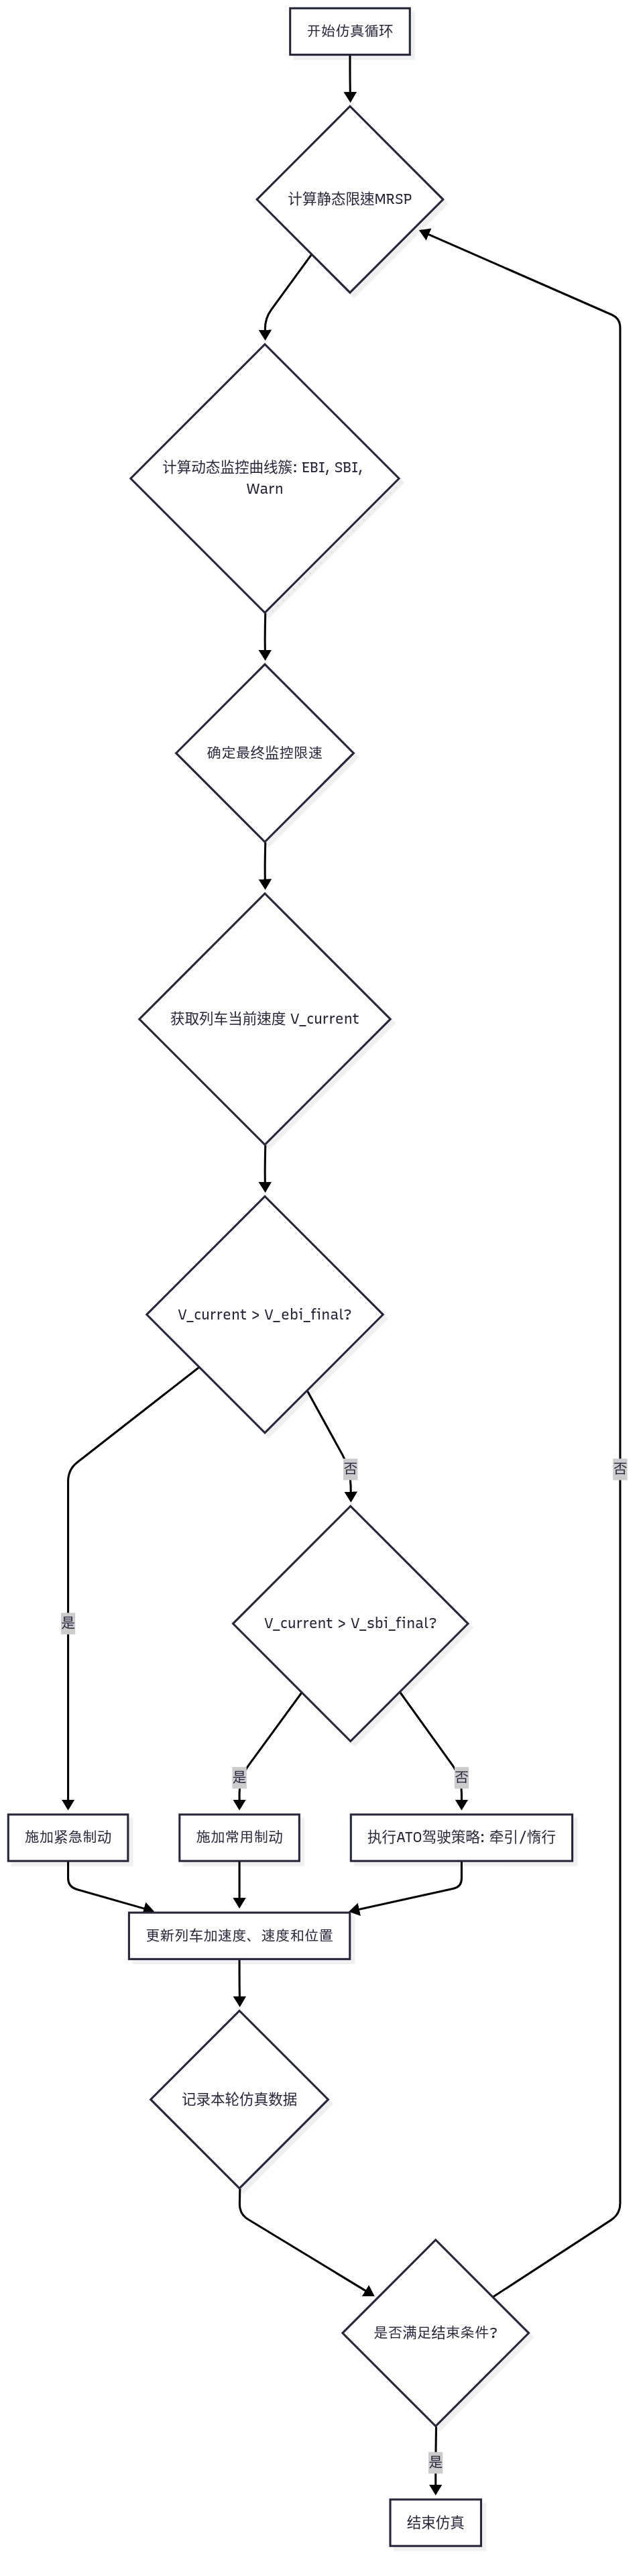
\includegraphics[width=0.7\textwidth,height=0.6\textheight,keepaspectratio]{flowchart_atp_loop.png}
    \caption{ATP速度监控主循环流程图}
    \label{fig:atp_loop}
\end{figure}

图\ref{fig:ato_strategy}则细化了在ATP安全框架下,两种不同驾驶策略的具体判断逻辑。

\begin{figure}[h!]
    \centering
    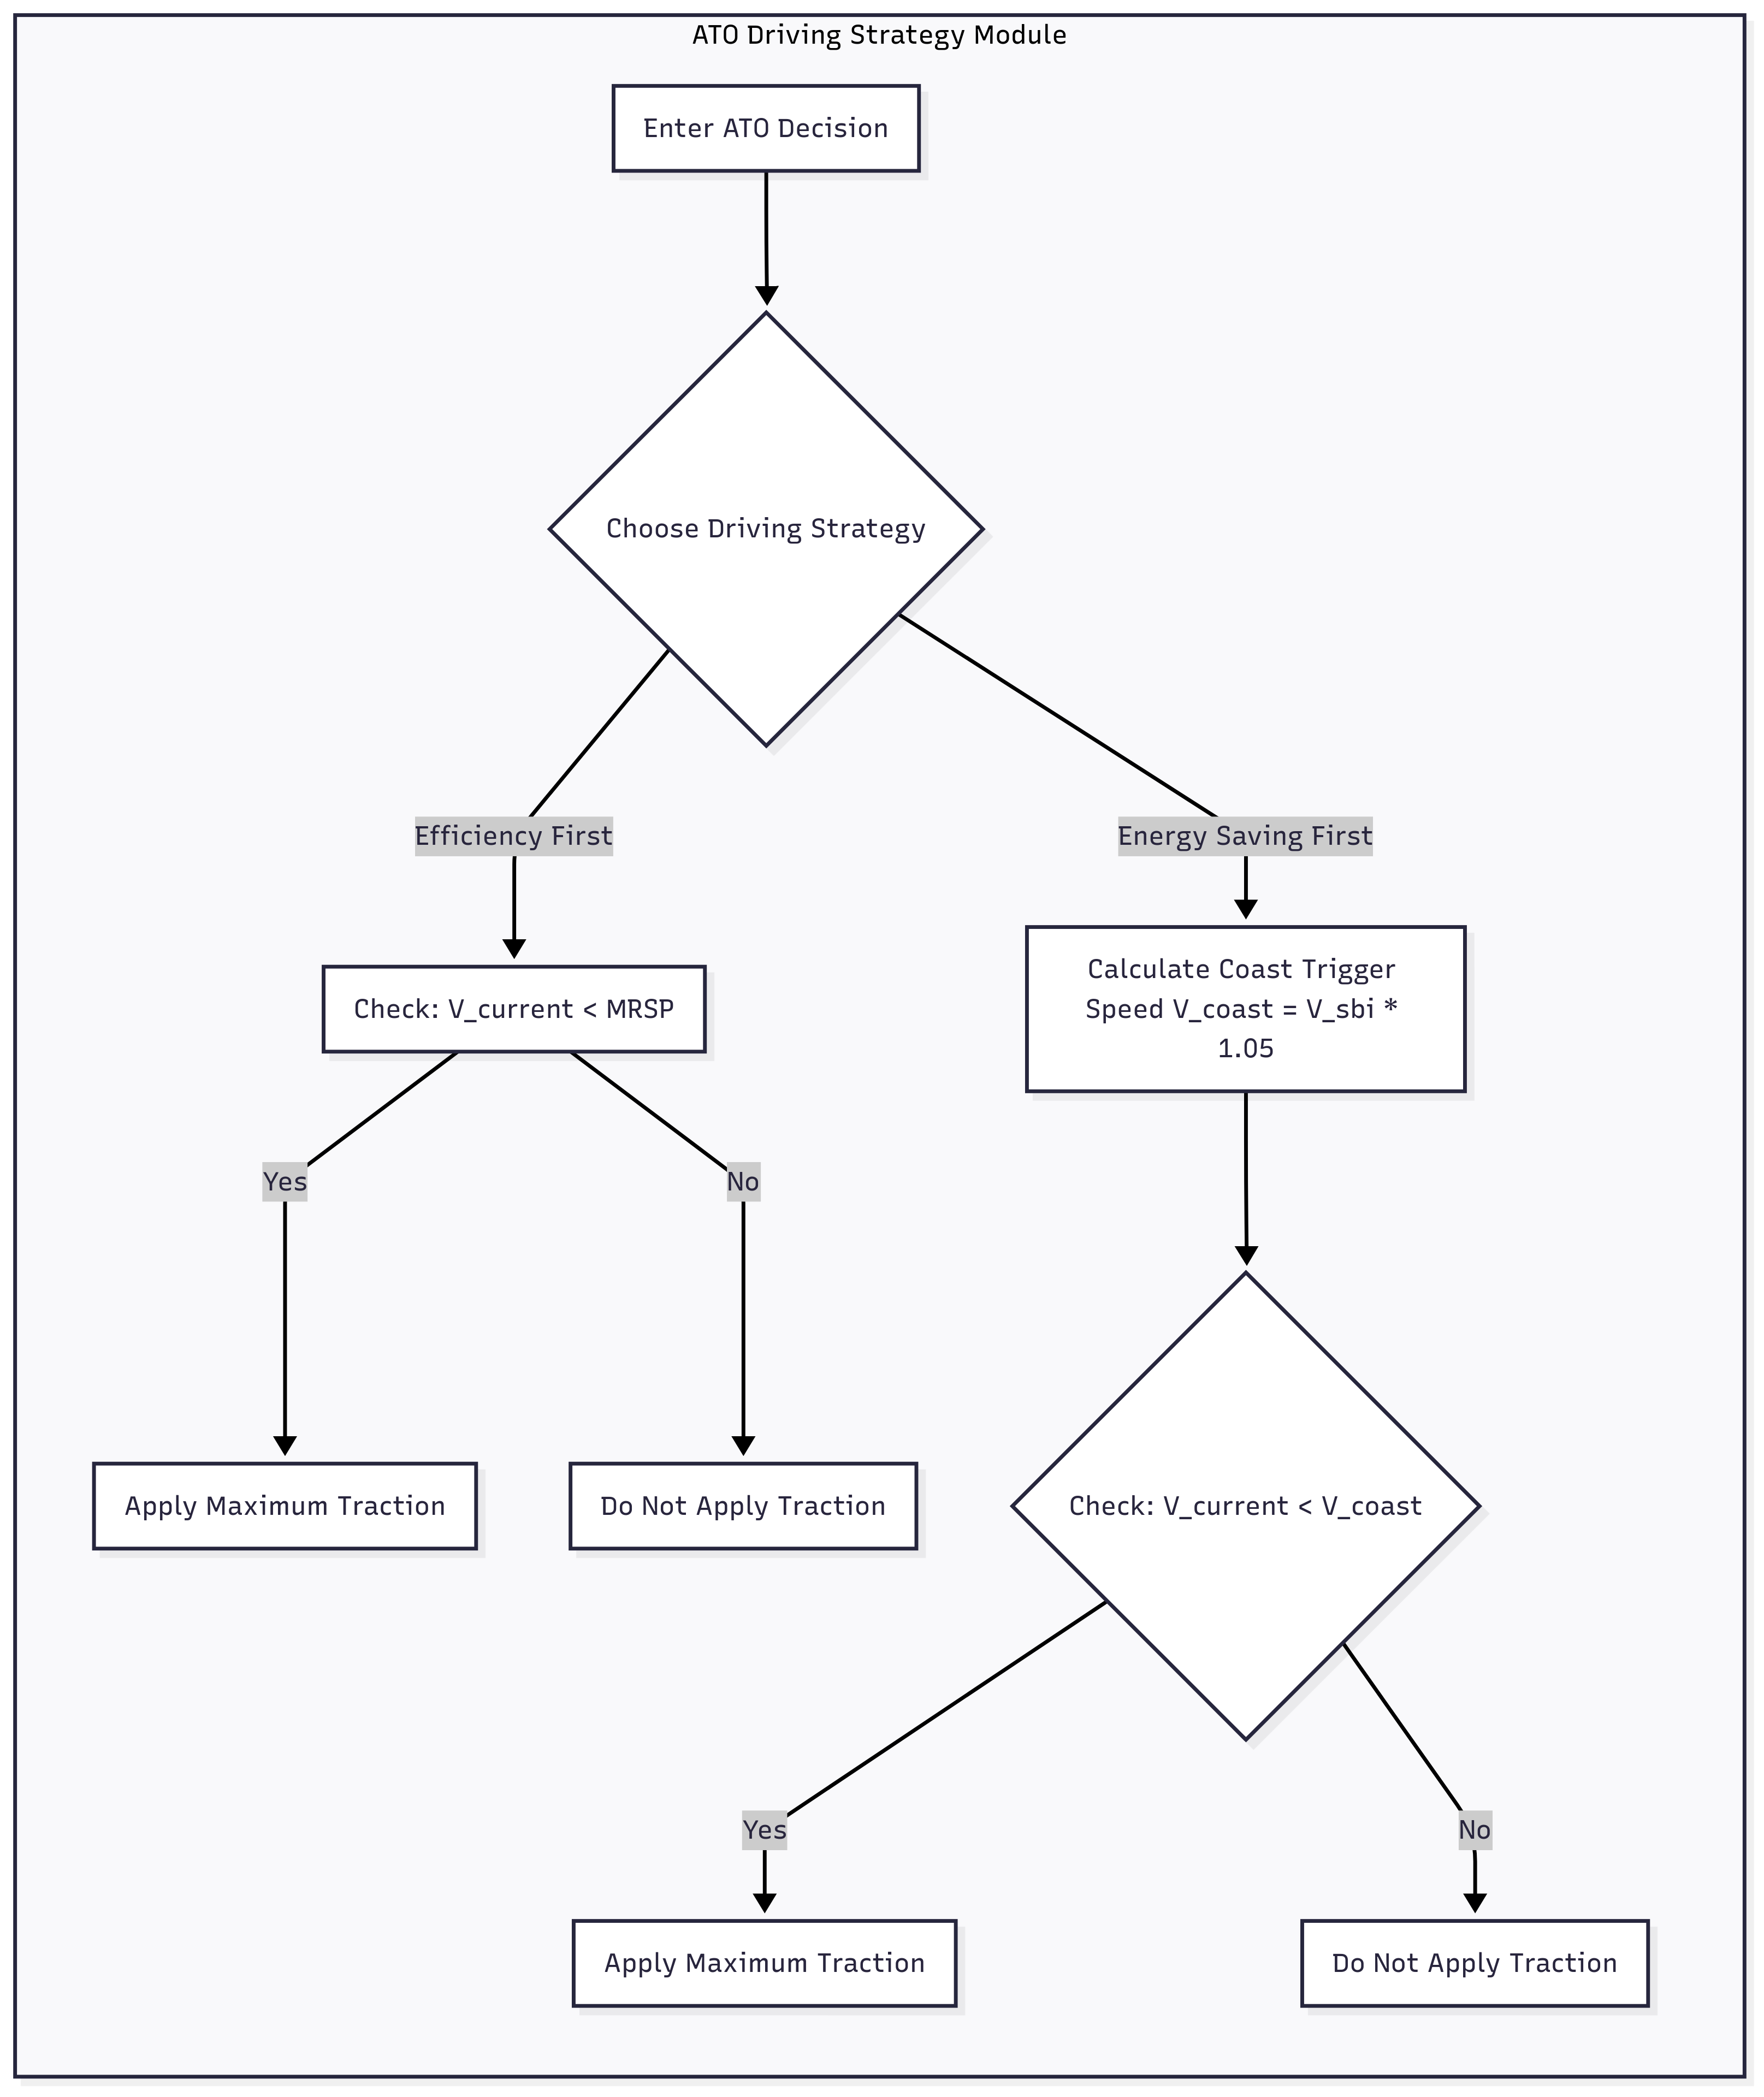
\includegraphics[width=0.7\textwidth]{flowchart_ato_strategy.png}
    \caption{ATO驾驶策略决策模型流程图}
    \label{fig:ato_strategy}
\end{figure}


% --- 结果与分析 ---
\section{结果与分析}
本章节将对三个核心仿真实验的结果进行详细的展示和分析。

\subsection{基础ATP与ATO策略仿真分析}
本实验首先对单列车在包含临时限速区的复杂场景下运行进行仿真,并对比了“效率优先”与“节能优先”两种ATO策略。

\begin{figure}[h!]
    \centering
    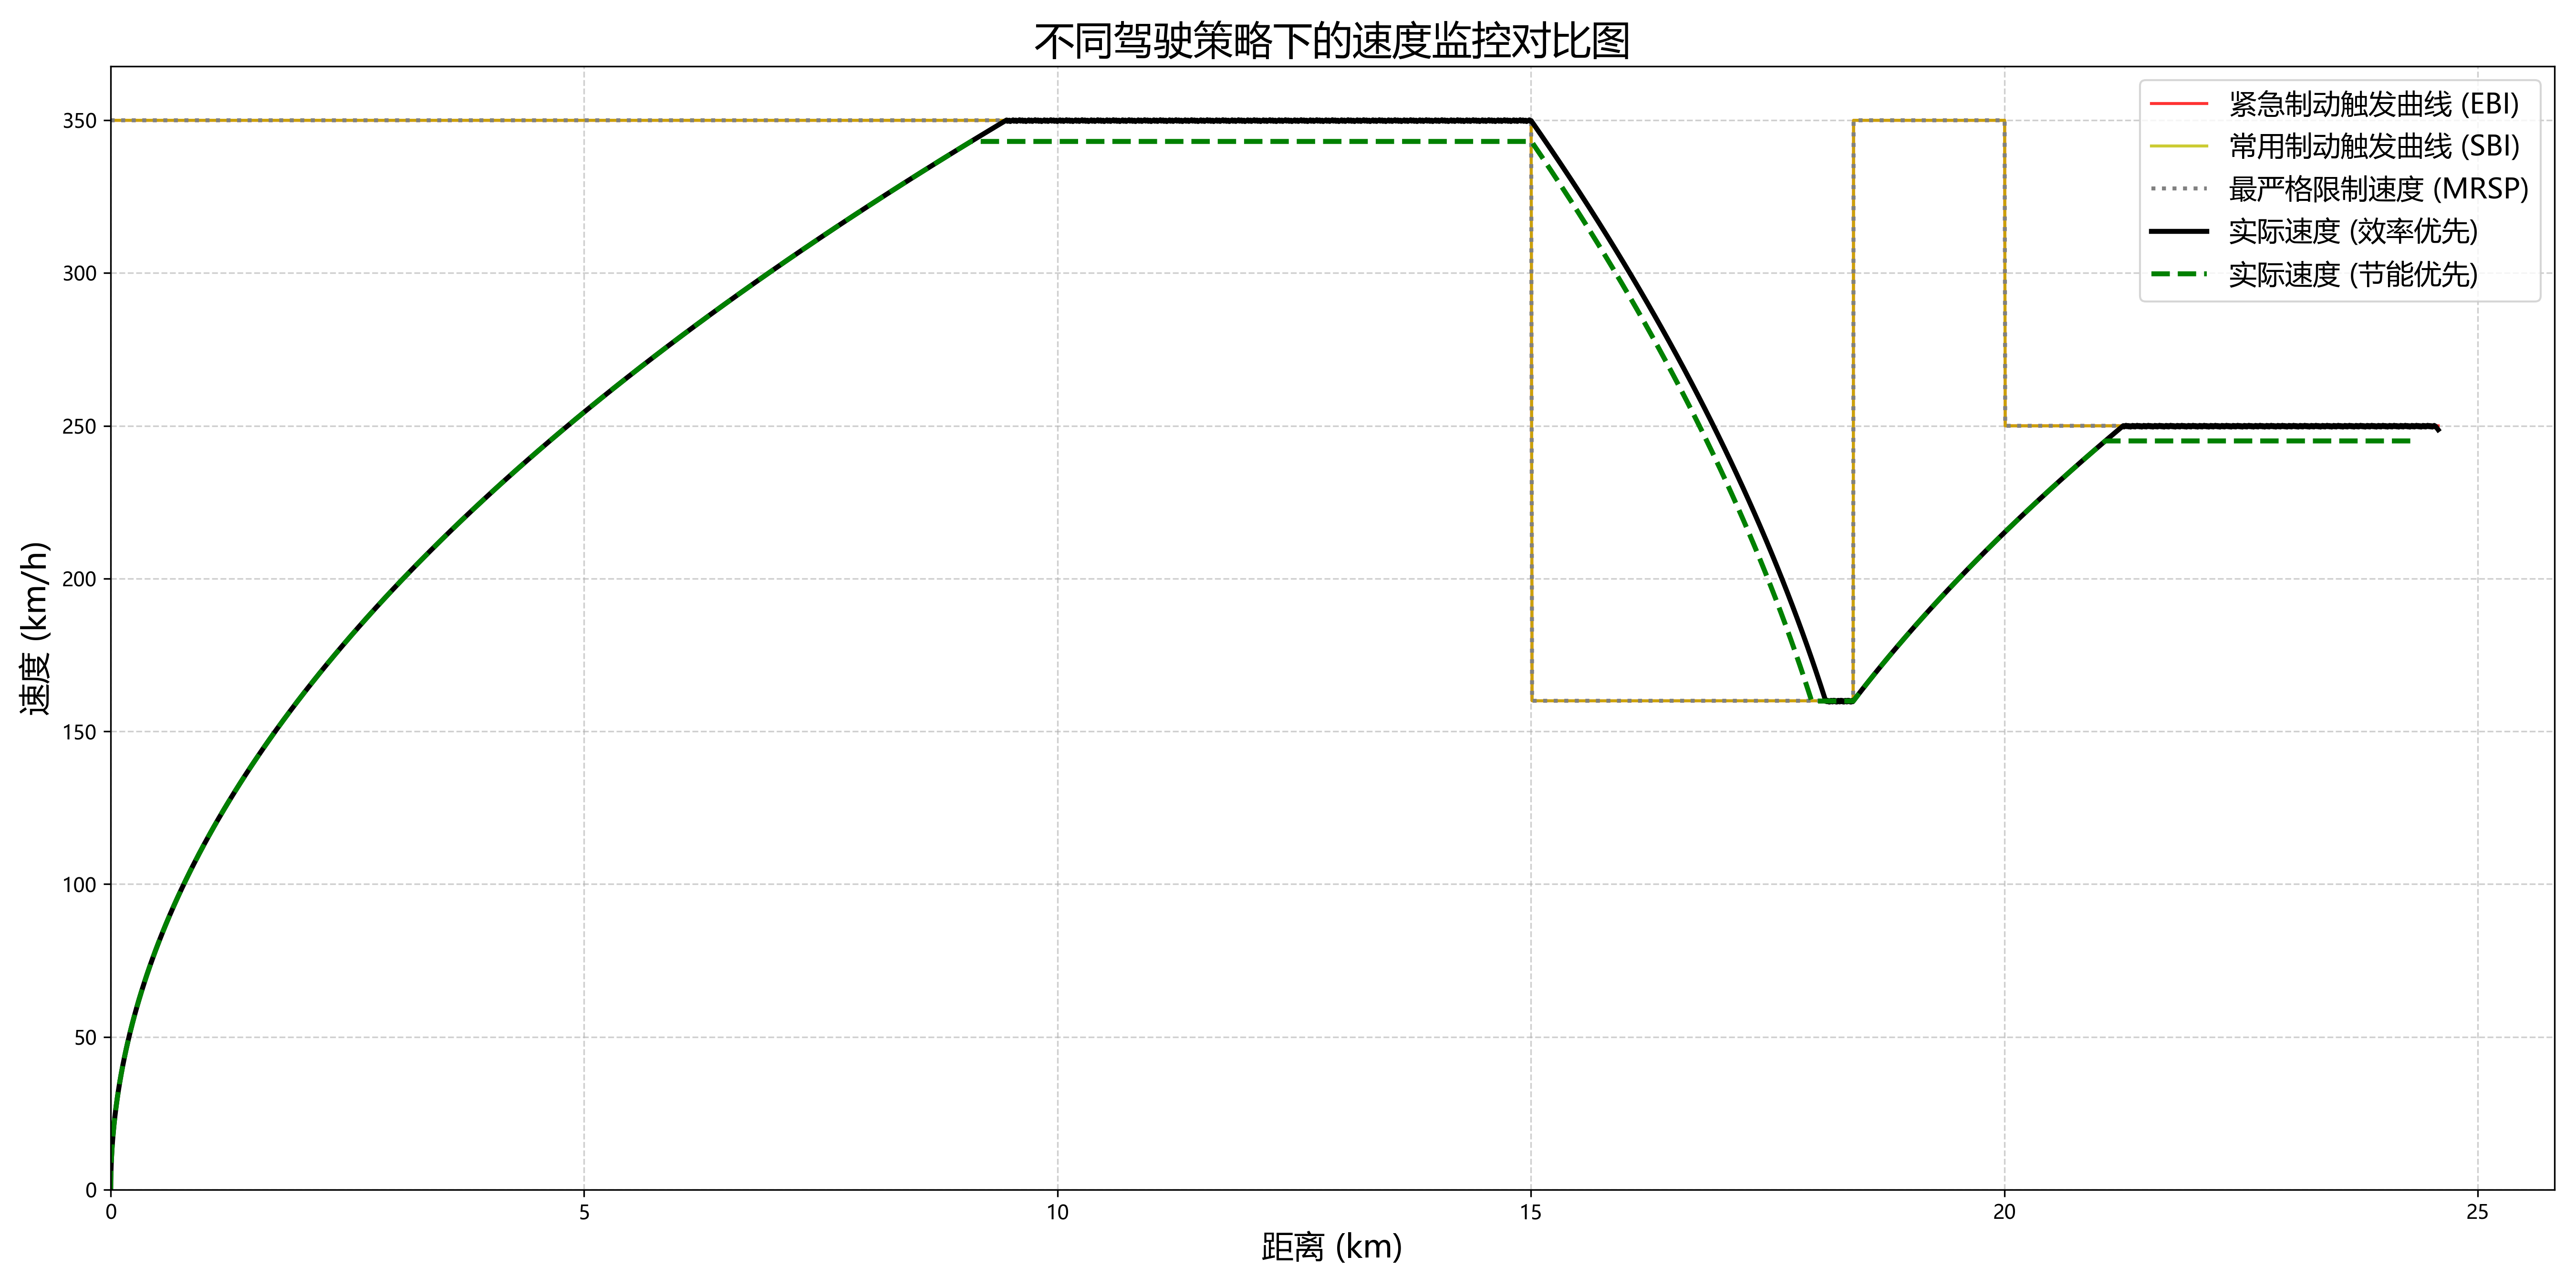
\includegraphics[width=\textwidth]{velocity_comparison_chart.png}
    \caption{不同驾驶策略下的速度监控对比图}
    \label{fig:velocity_comparison}
\end{figure}

\begin{figure}[h!]
    \centering
    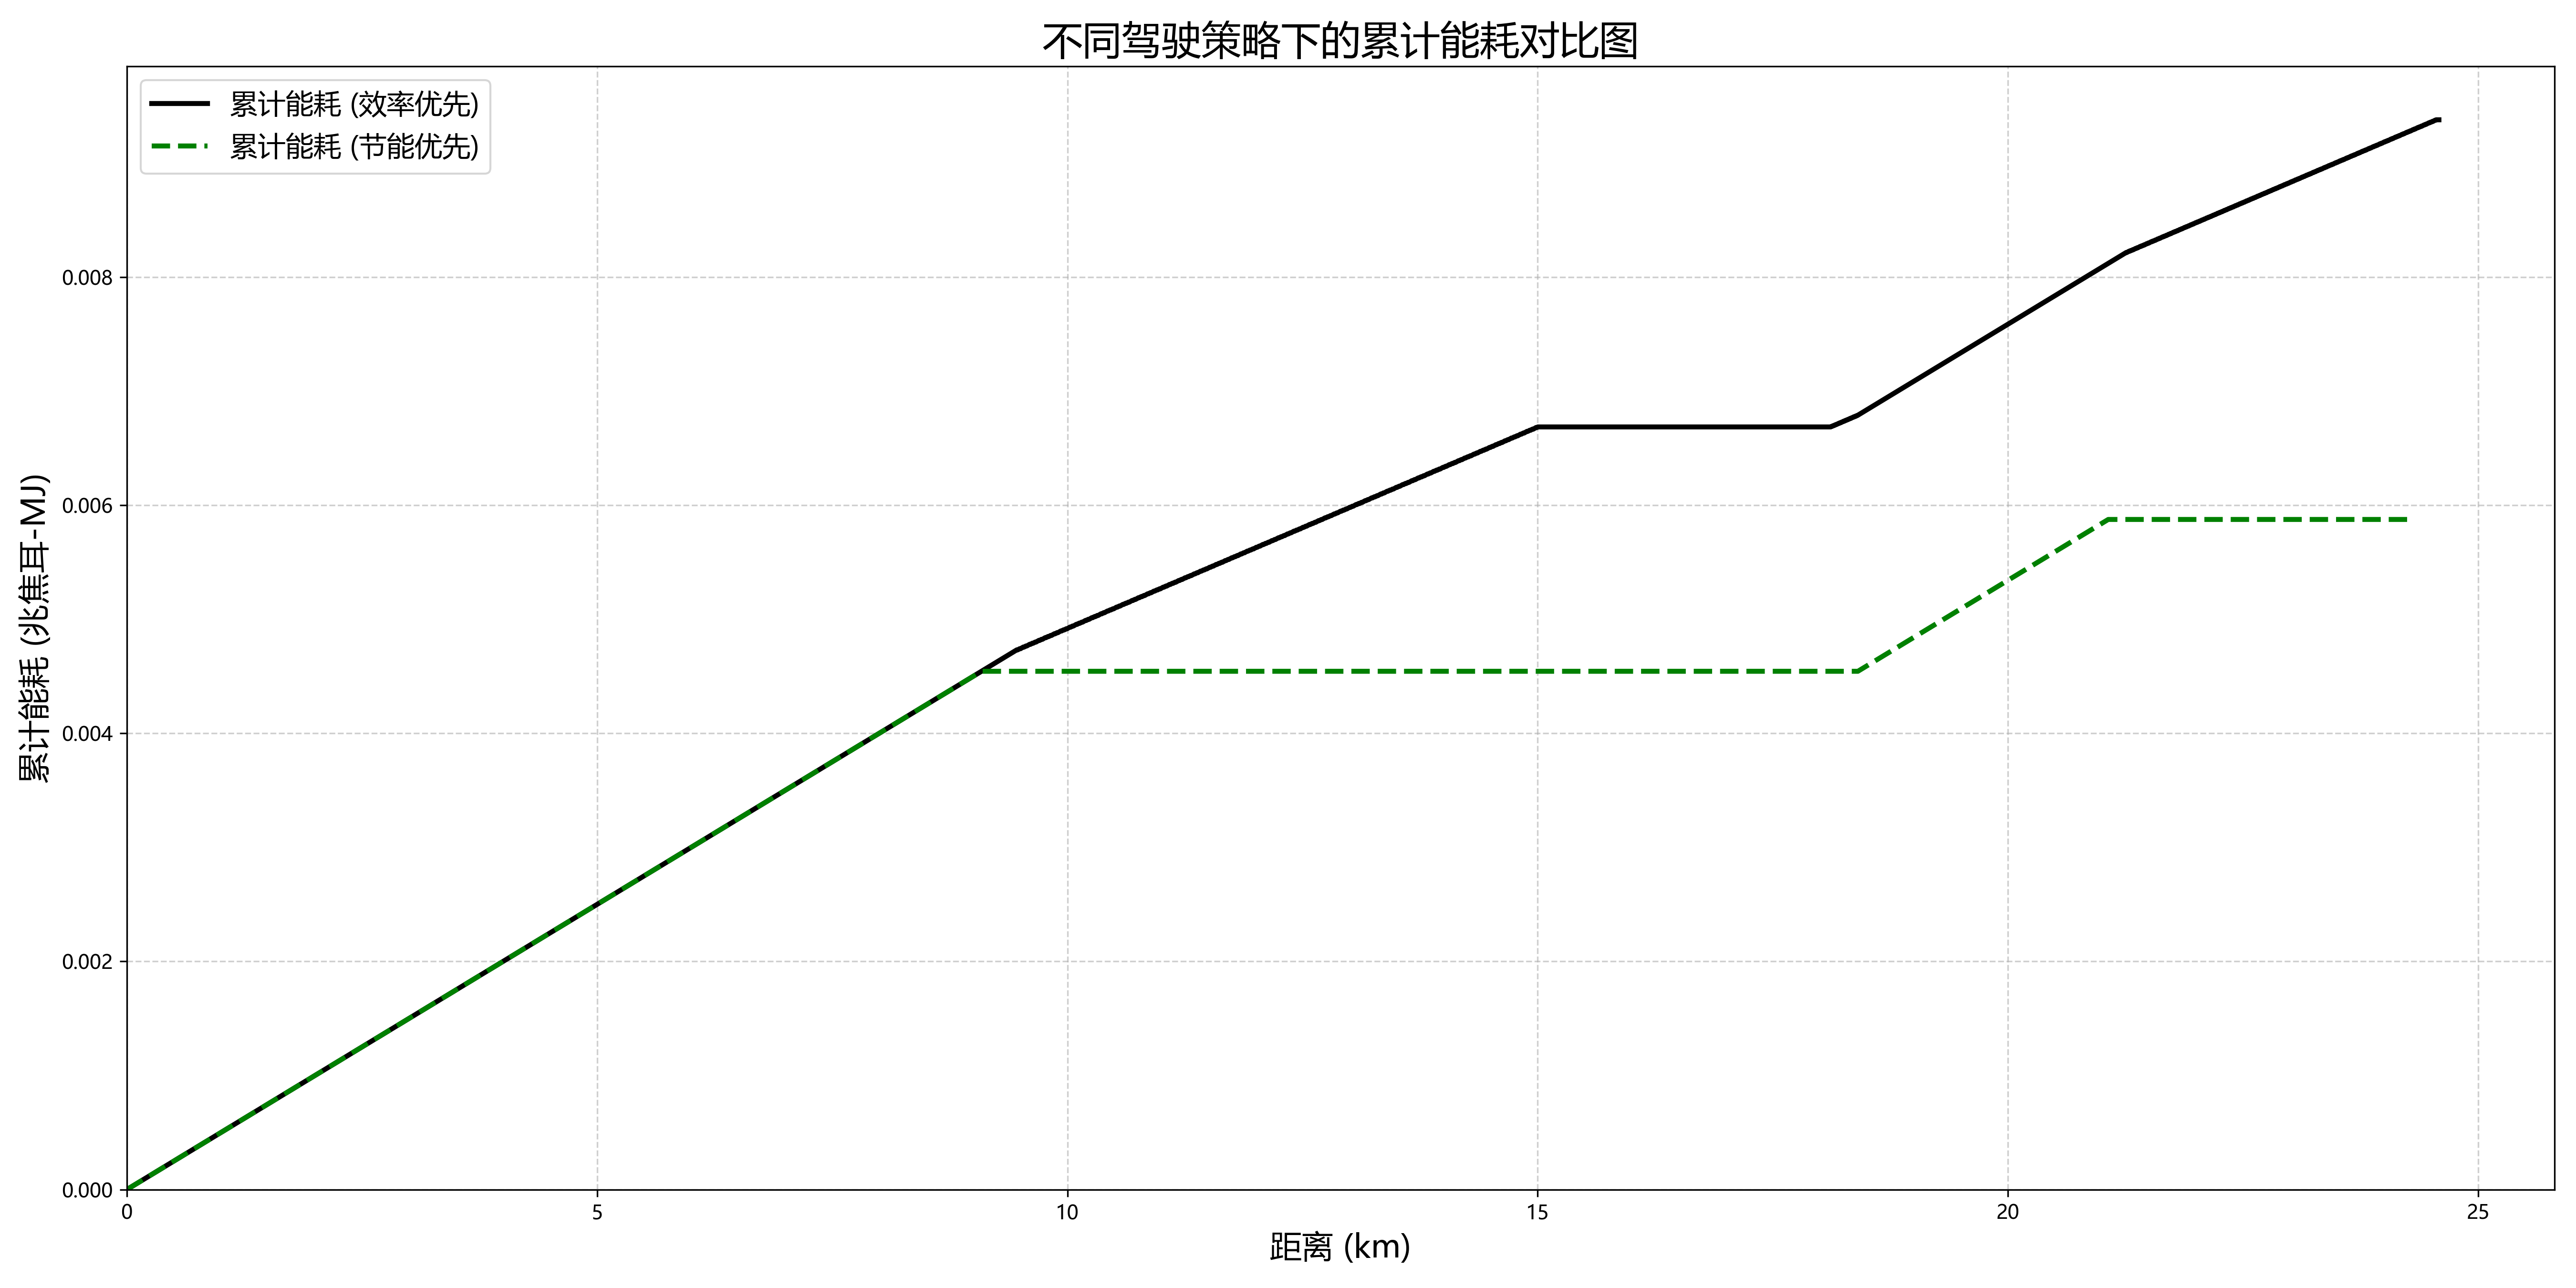
\includegraphics[width=\textwidth]{energy_comparison_chart.png}
    \caption{不同驾驶策略下的累计能耗对比图}
    \label{fig:energy_comparison}
\end{figure}

从图\ref{fig:velocity_comparison}可以看出,两种策略的运行轨迹均被ATP安全包络(由EBI、SBI、MRSP曲线构成)完美地保护。在18km处驶出临时限速区后,两种策略出现显著分化:“效率优先”策略(黑色实线)立即以最大功率加速,试图尽快达到250km/h的线路限速;而“节能优先”策略(绿色虚线)则判断出无需再次加速,通过长时间的惰行来为最终的停车目标做准备。

图\ref{fig:energy_comparison}量化了这种差异。在18km后,“效率优先”策略的能耗曲线斜率陡增,表明其进行了高功率的牵引。相比之下,“节能优先”策略的能耗曲线几乎变为水平,表明其处于零能耗的惰行状态。最终,节能策略以牺牲少量运行时间为代价,显著降低了总能耗。

\subsection{CTCS-3级动态授权仿真分析}
本实验模拟了CTCS-3级下列车与RBC的交互过程,其核心交互模型如图\ref{fig:ctcs3_model}所示,具体流程如图\ref{fig:ma_update}所示。

\begin{figure}[h!]
    \centering
    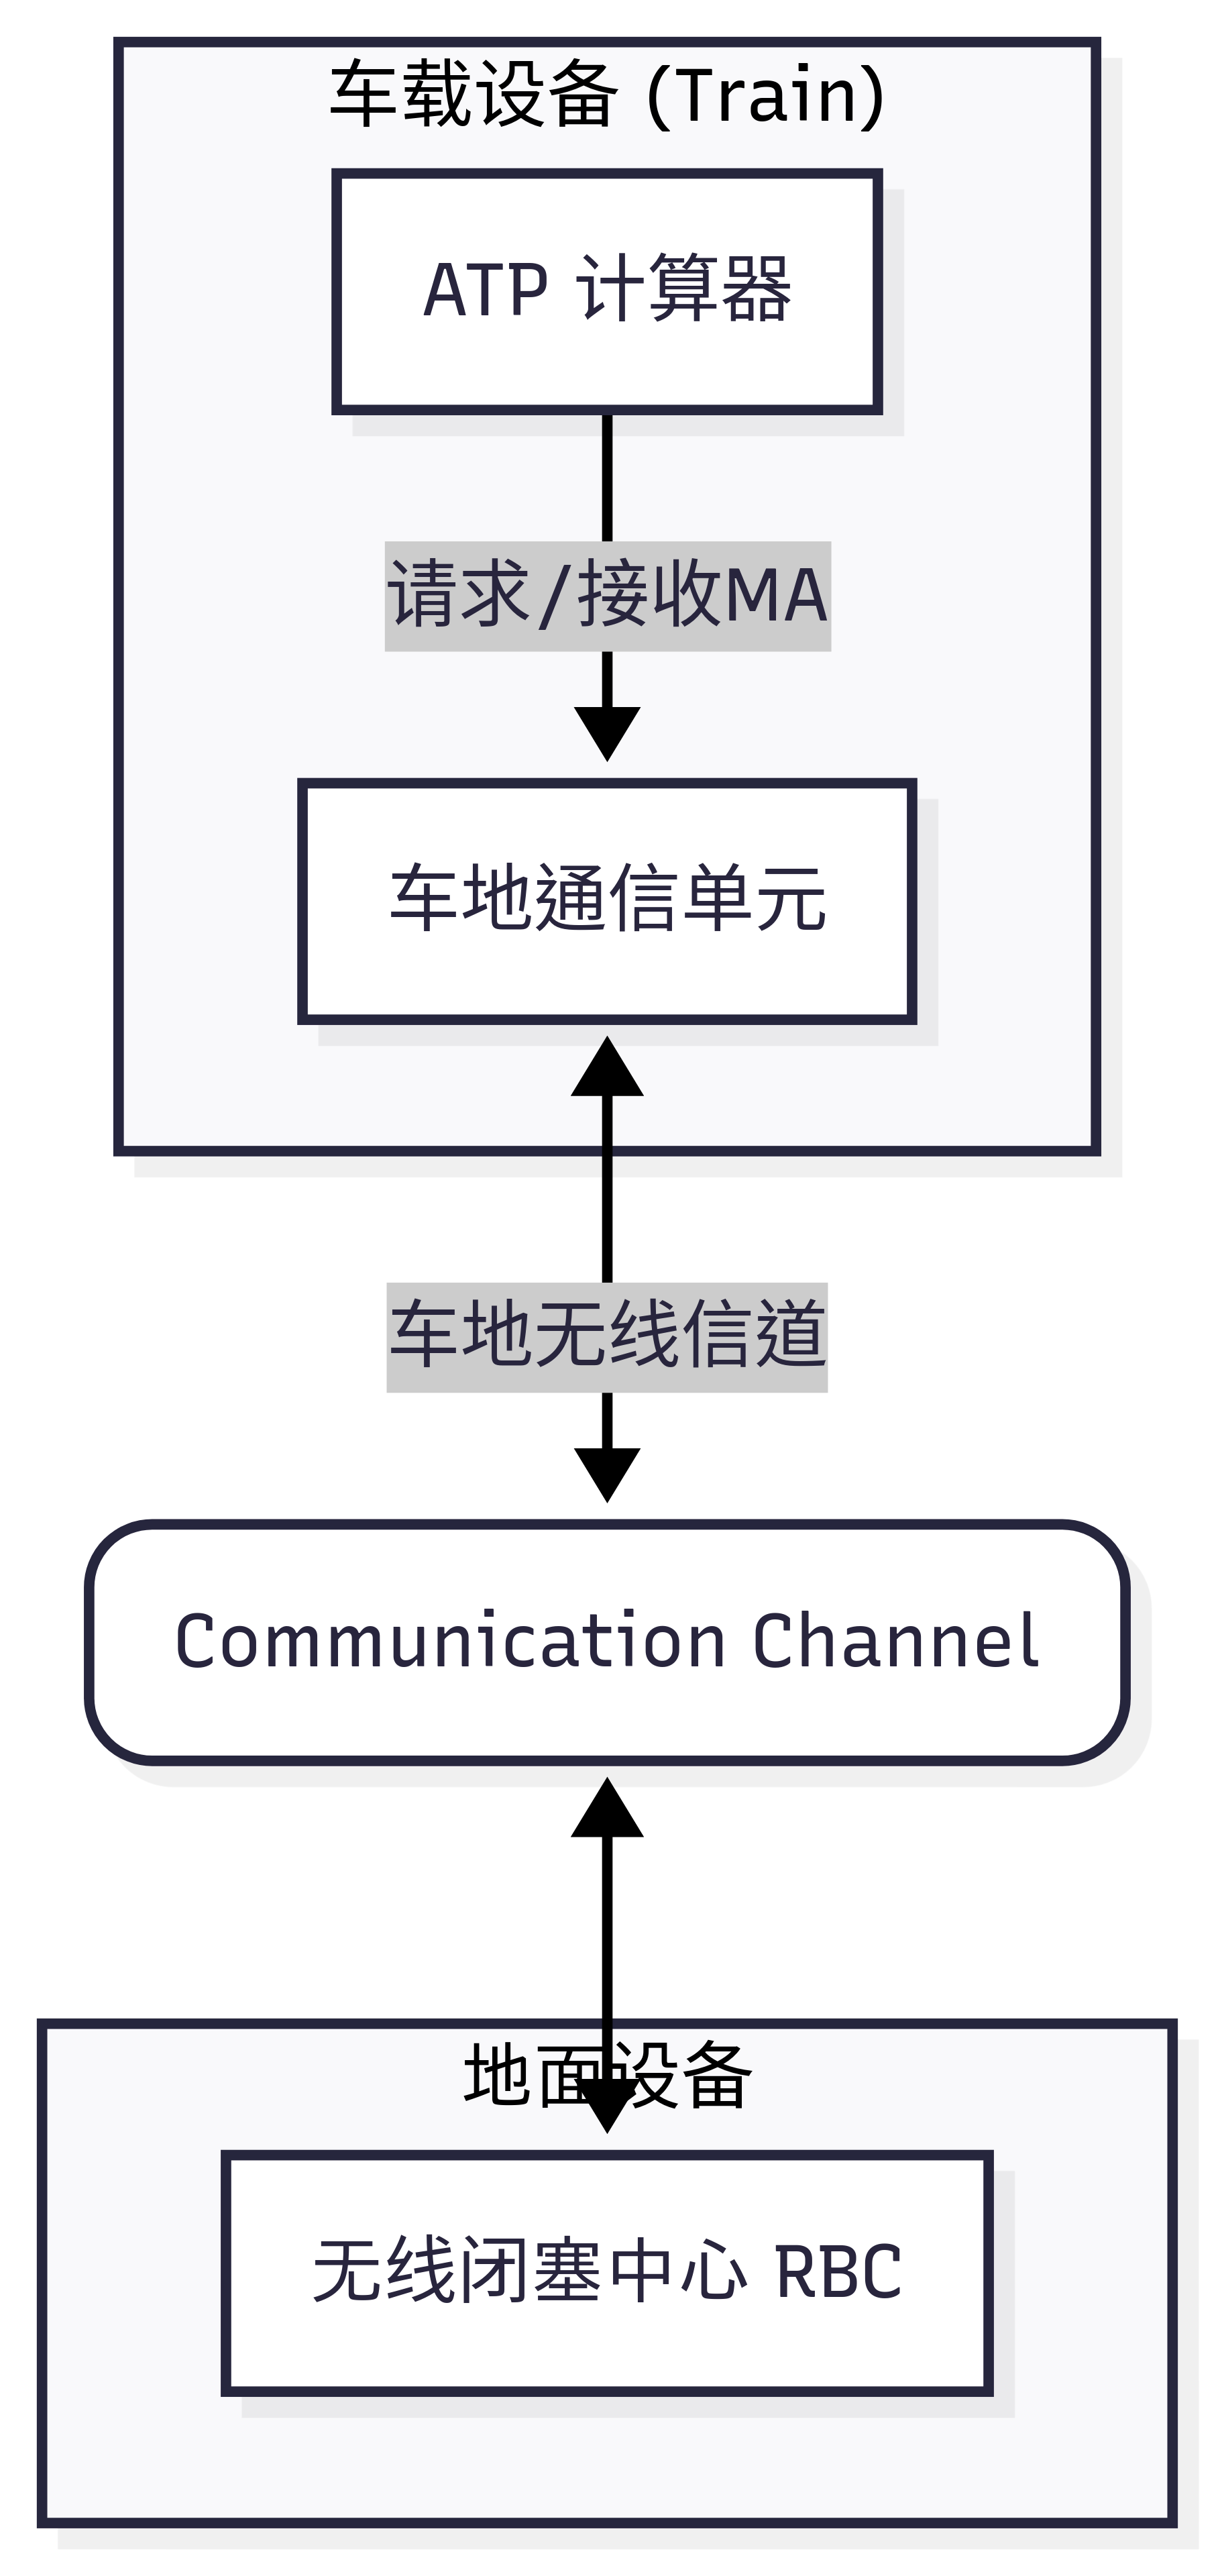
\includegraphics[width=0.6\textwidth,height=0.6\textheight,keepaspectratio]{flowchart_ctcs3_model.png}
    \caption{CTCS-3级系统简化模型示意图}
    \label{fig:ctcs3_model}
\end{figure}

\begin{figure}[h!]
    \centering
    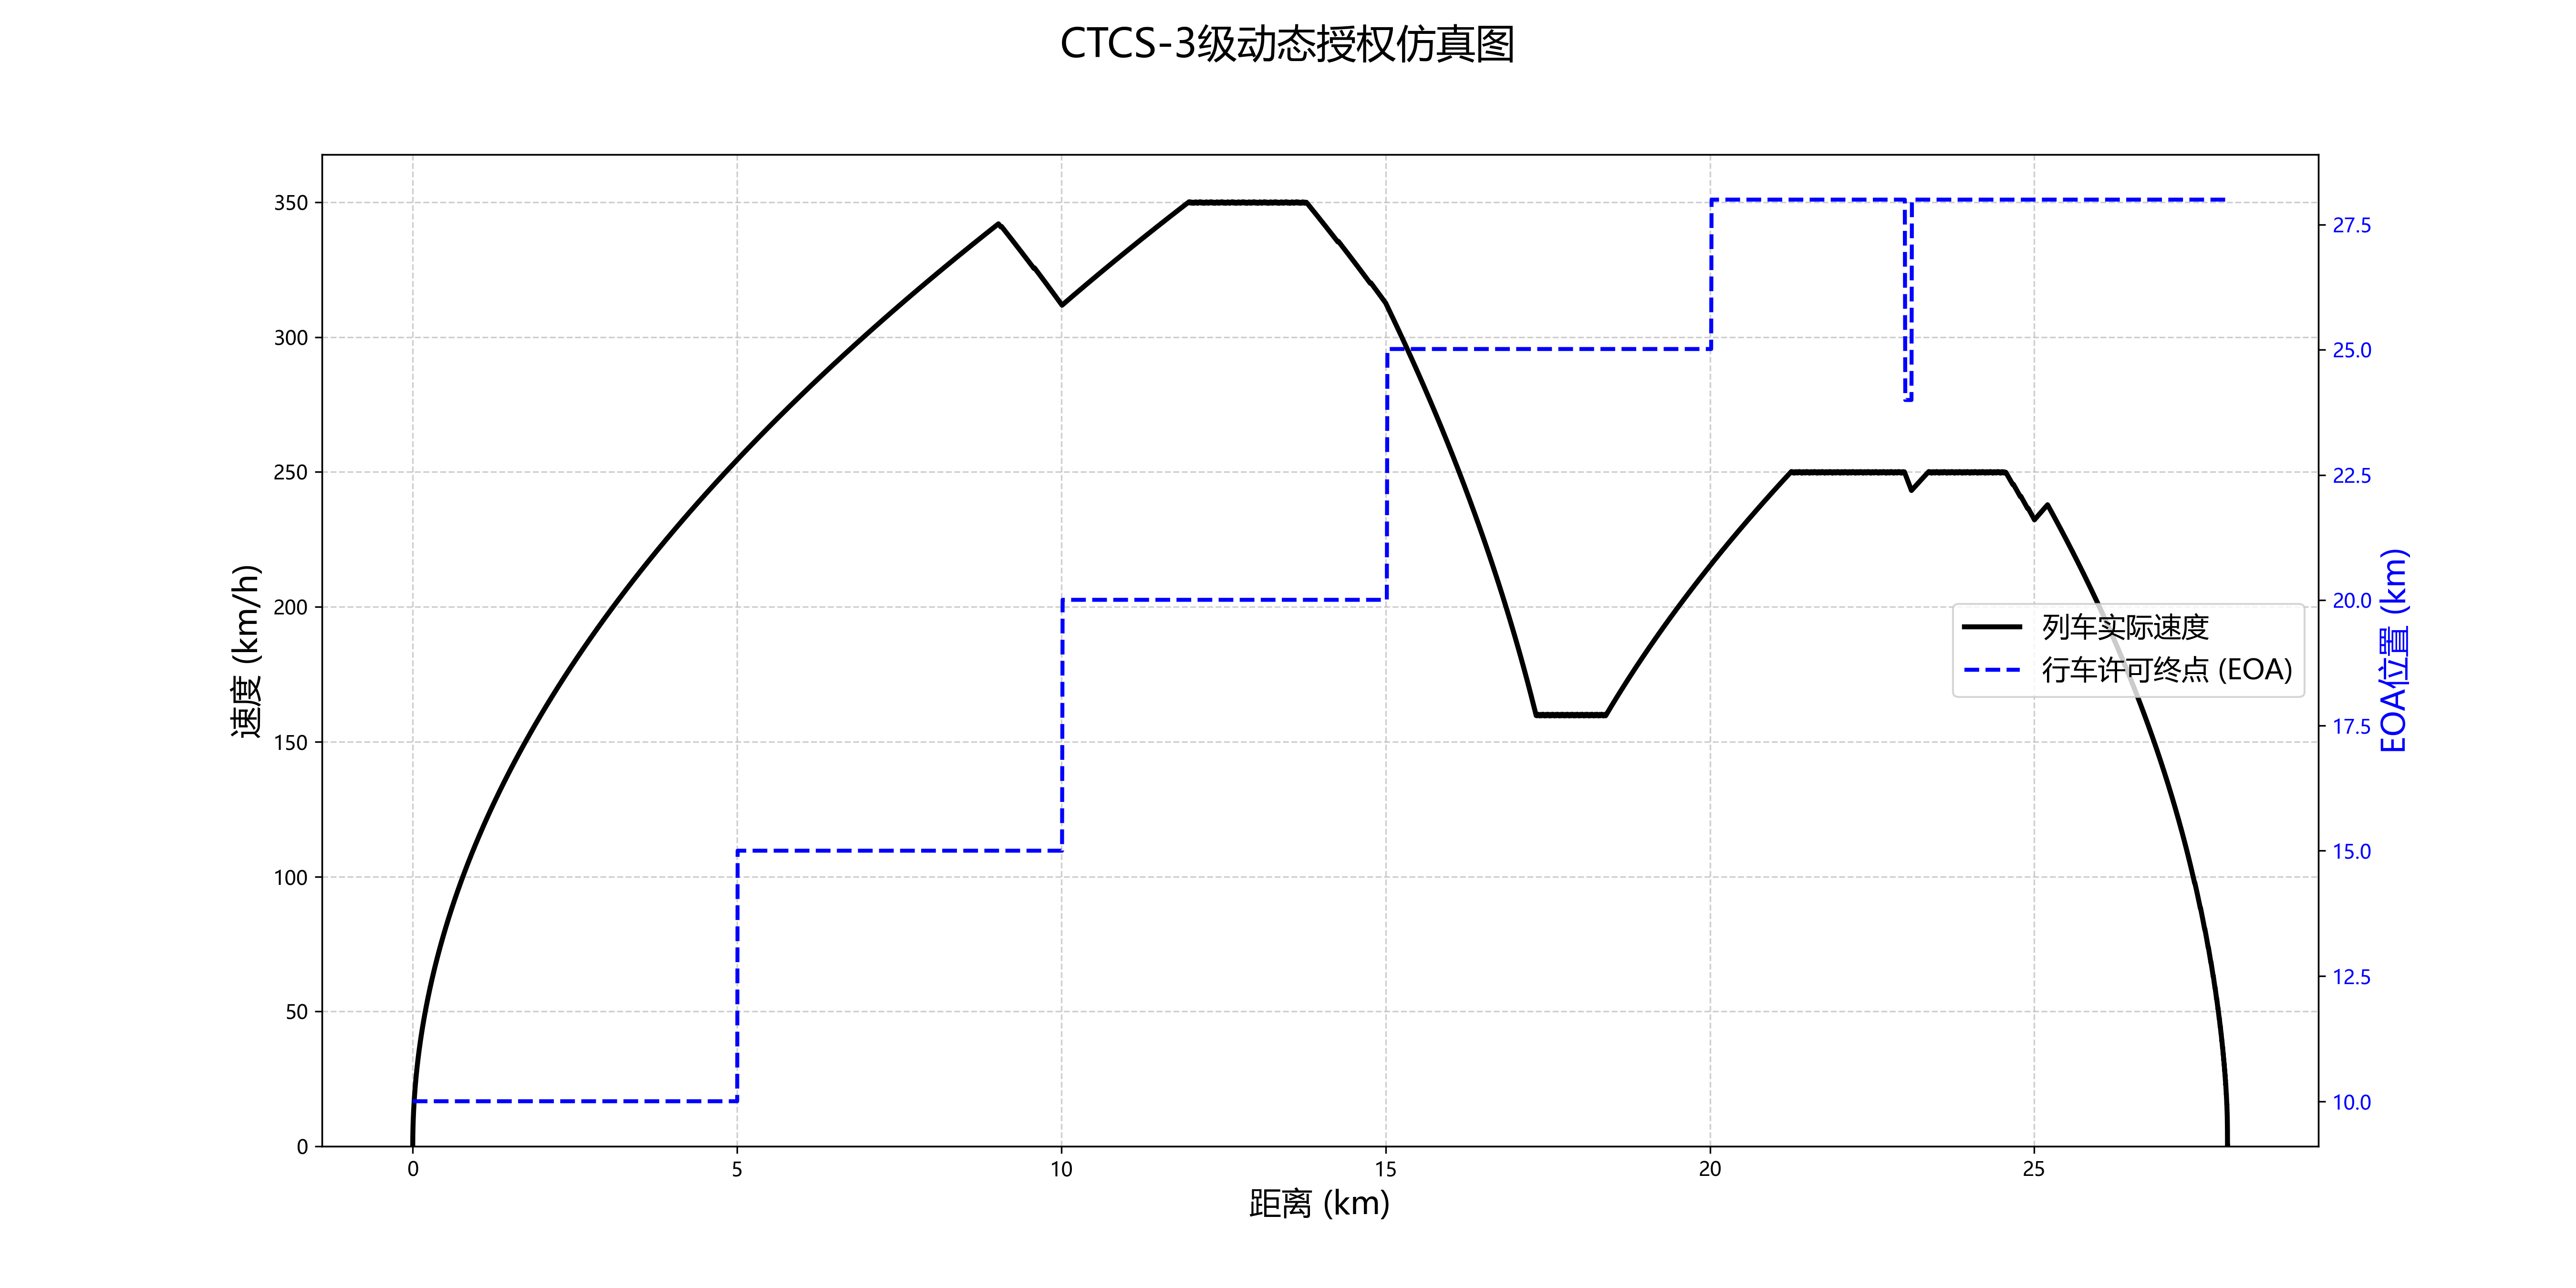
\includegraphics[width=\textwidth]{c3_simulation_chart.png}
    \caption{CTCS-3级动态授权仿真图}
    \label{fig:c3_simulation}
\end{figure}

如图\ref{fig:c3_simulation}所示,行车许可终点(EOA,蓝色虚线)并非固定不变,而是在列车运行过程中呈阶梯状向前延伸。当列车接近当前的EOA时(约5km, 15km处),车载设备向RBC请求并获得了新的、更远的MA,使得列车可以不减速地持续高速运行。在23km处,仿真模拟了RBC下发紧急命令,将EOA从28km缩短至24km,列车ATP系统立即响应,触发了紧急制动,并安全地停在了新目标点之前。该结果成功验证了CTCS-3级动态授权的高效性与安全性。

\subsection{多列车追踪与行车间隔分析}
为探究最小安全行车间隔,本实验进行了一系列不同发车间隔下的双车追踪仿真,其仿真逻辑如图\ref{fig:multitrain_loop}所示。

\begin{figure}[h!]
    \centering
    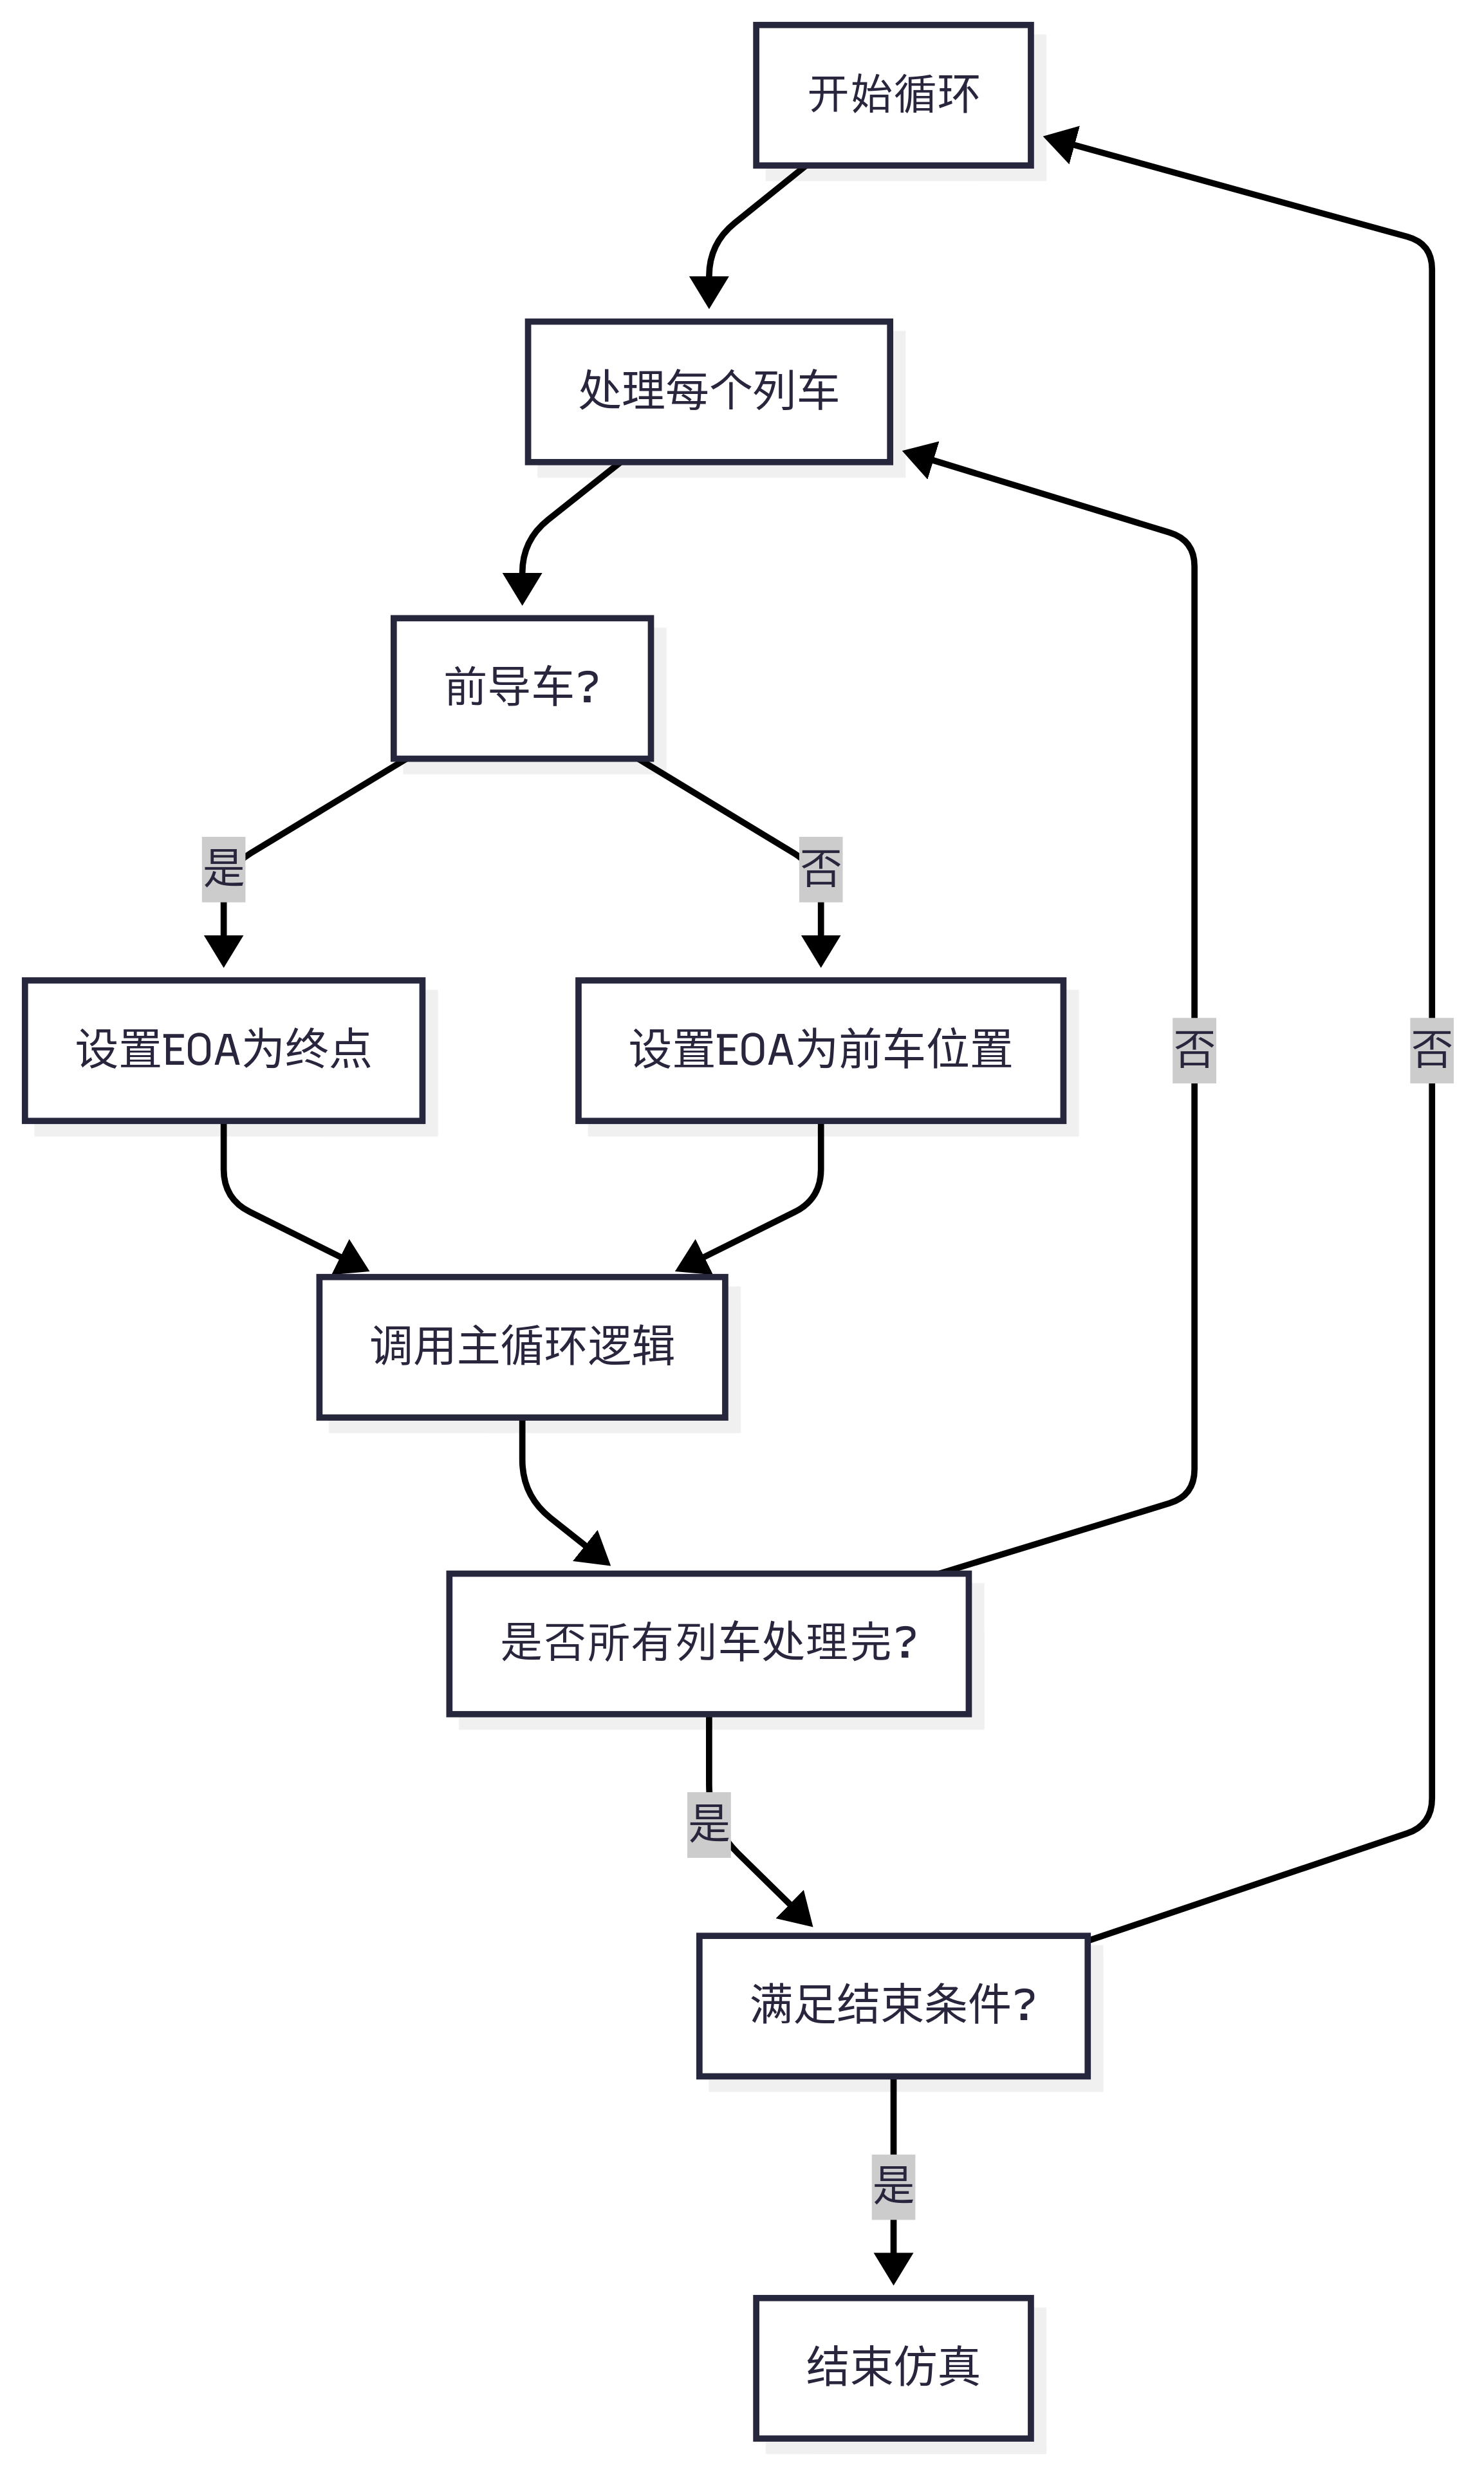
\includegraphics[width=0.7\textwidth]{flowchart_multitrain_loop.png}
    \caption{多列车追踪仿真主流程图}
    \label{fig:multitrain_loop}
\end{figure}

\begin{figure}[h!]
    \centering
    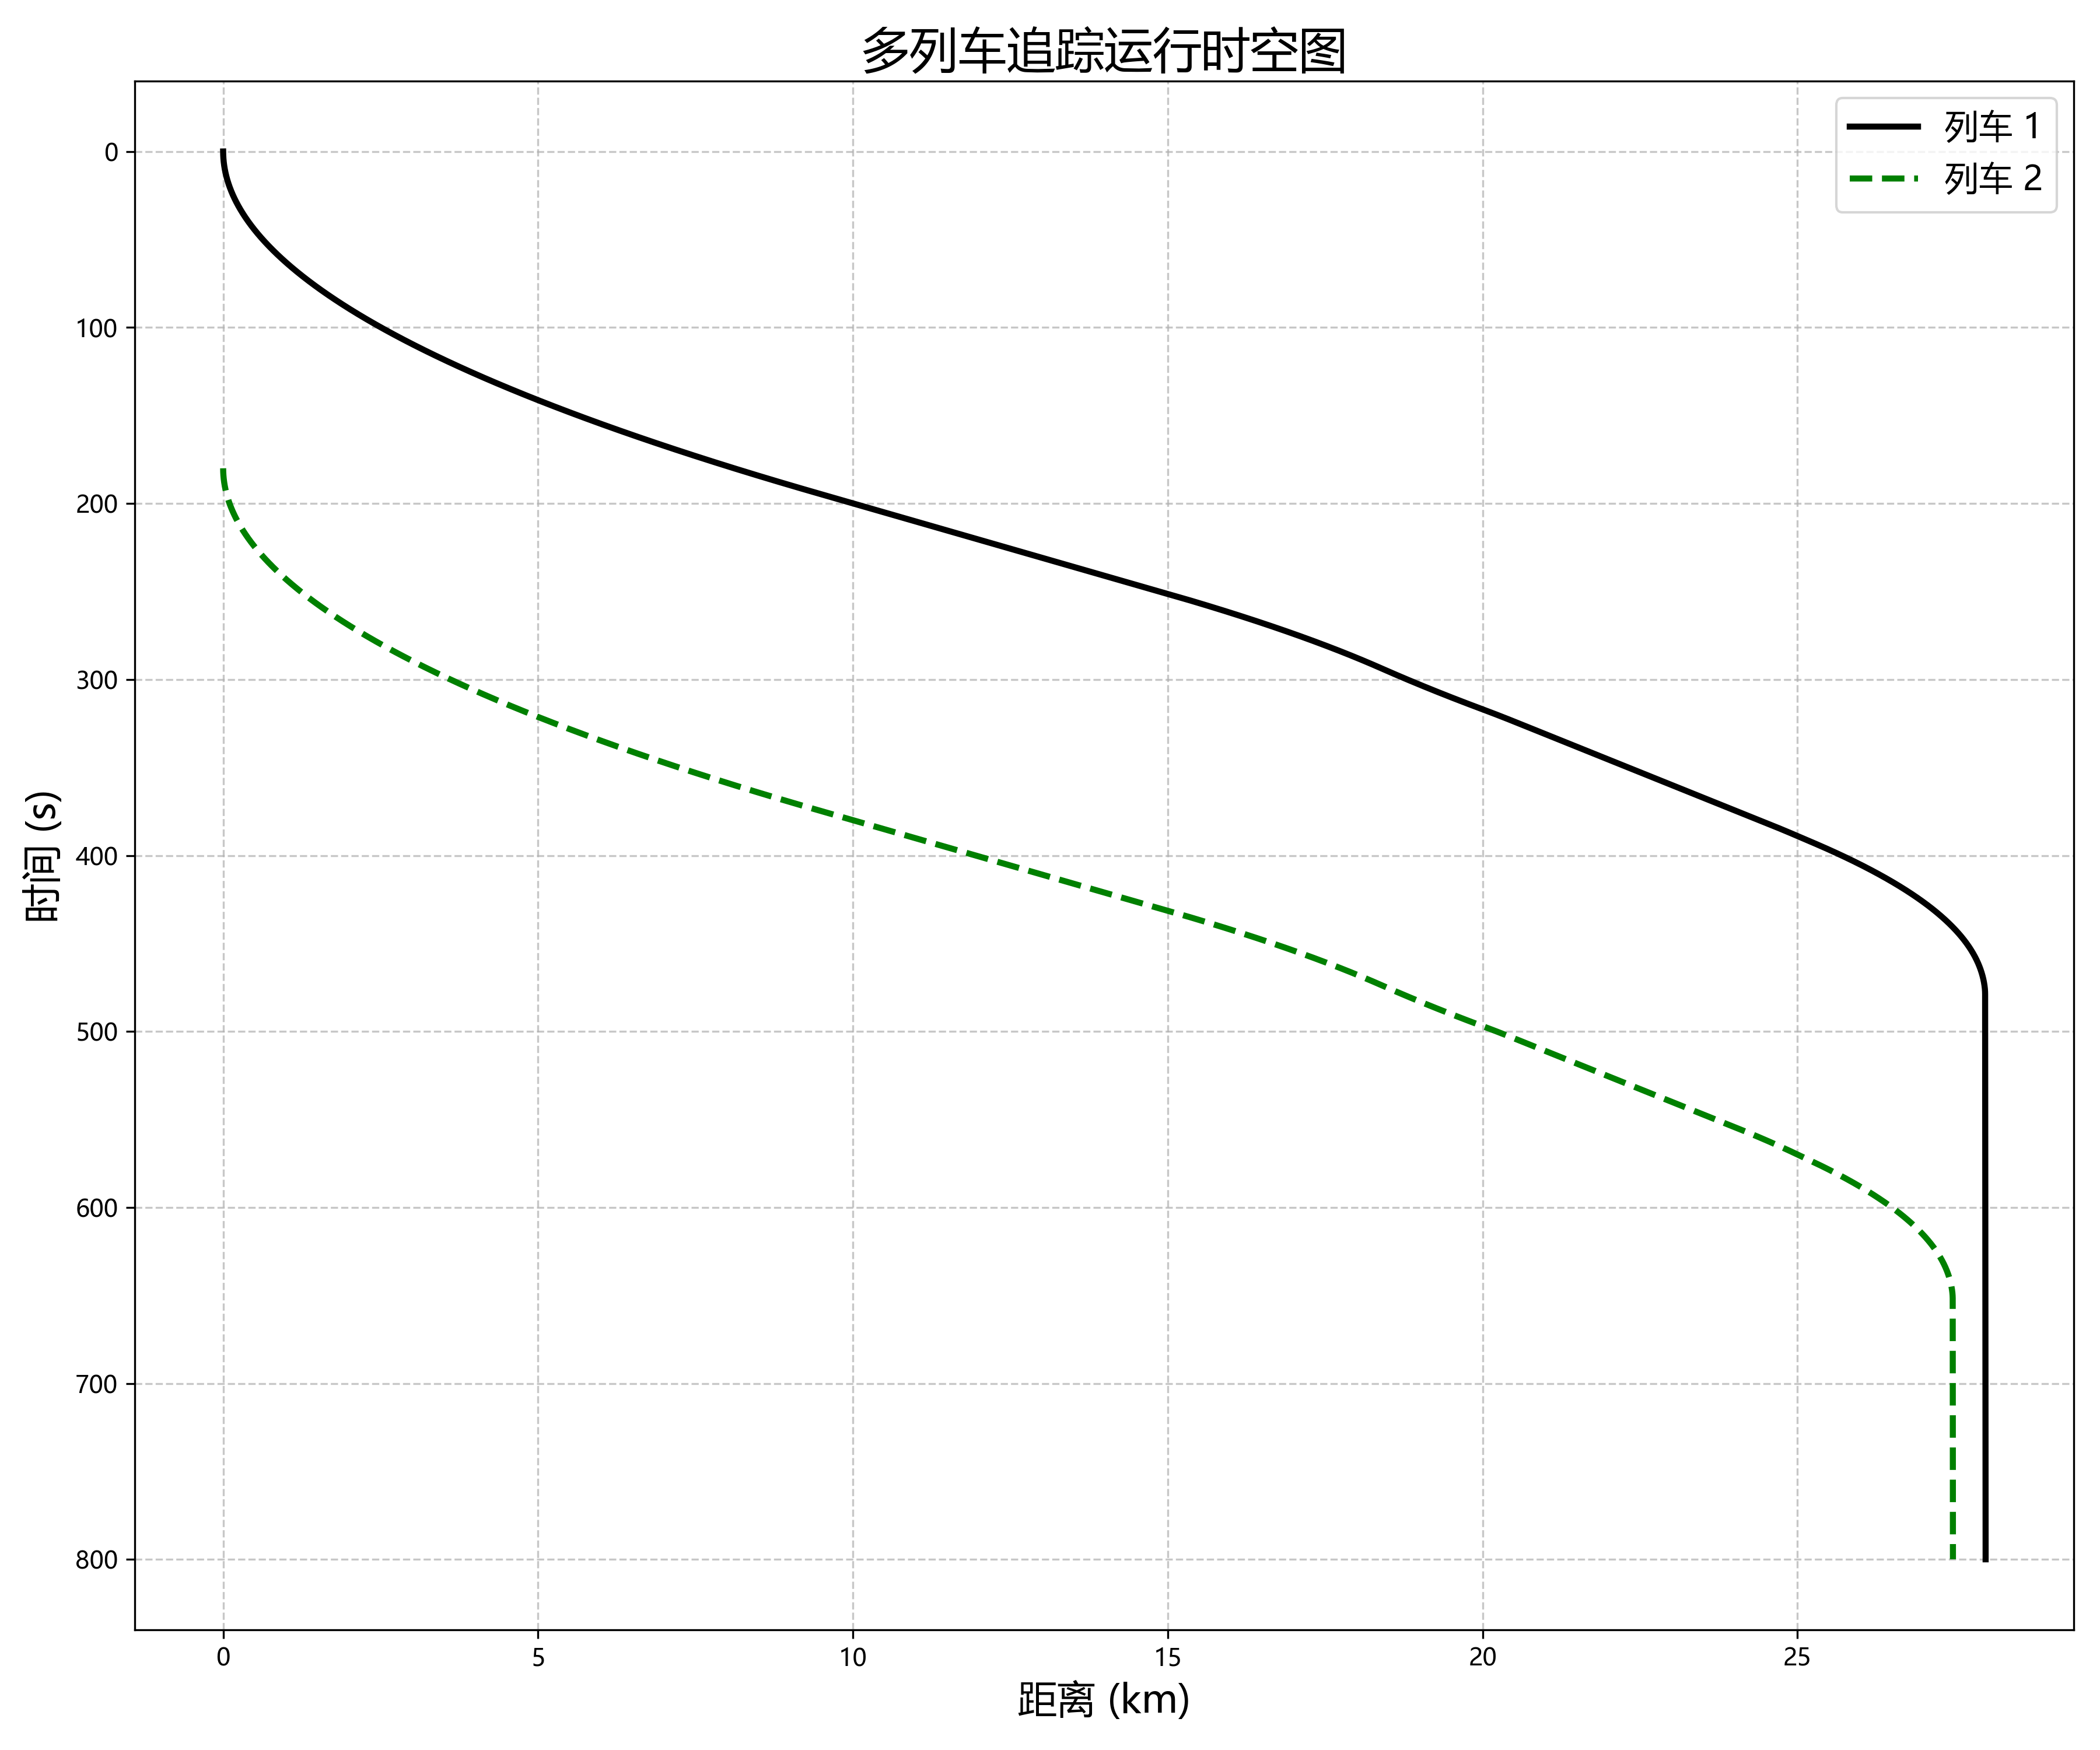
\includegraphics[width=0.48\textwidth]{headway_180s.png}
    \hfill
    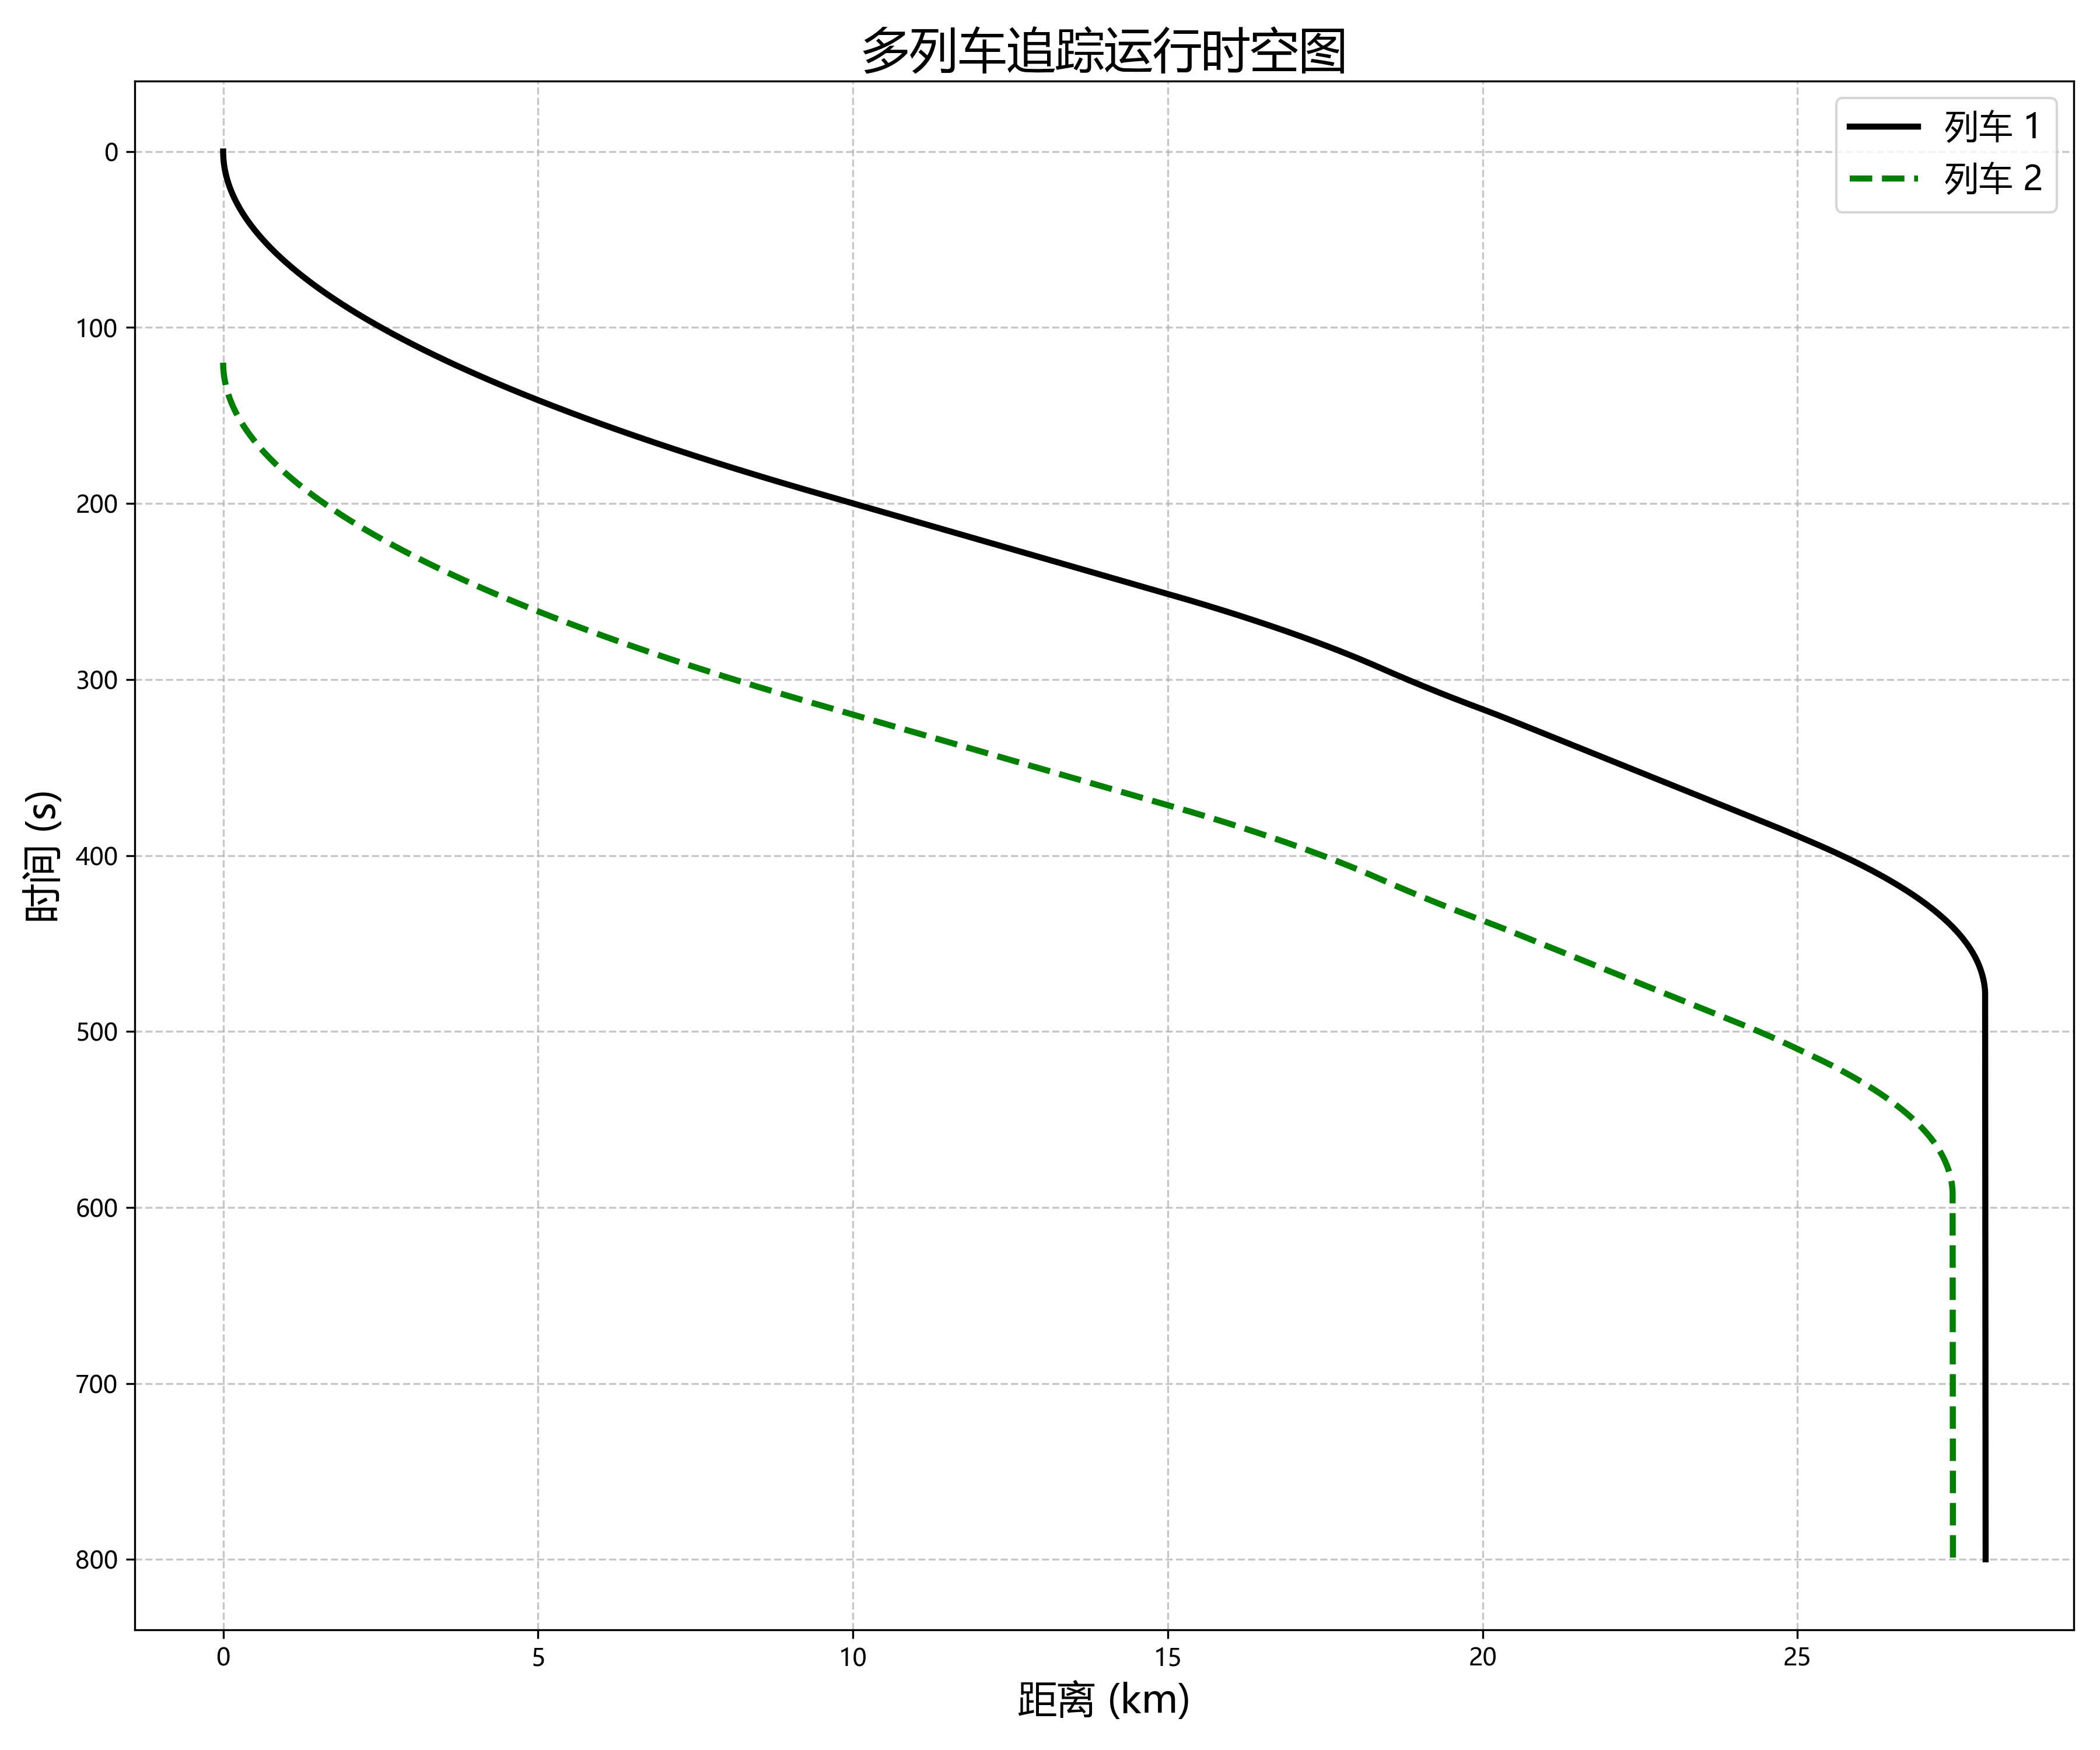
\includegraphics[width=0.48\textwidth]{headway_120s.png}
    \caption{宽松间隔(180s, 左)与临界间隔(120s, 右)时空图对比}
    \label{fig:headway_compare1}
\end{figure}

\begin{figure}[h!]
    \centering
    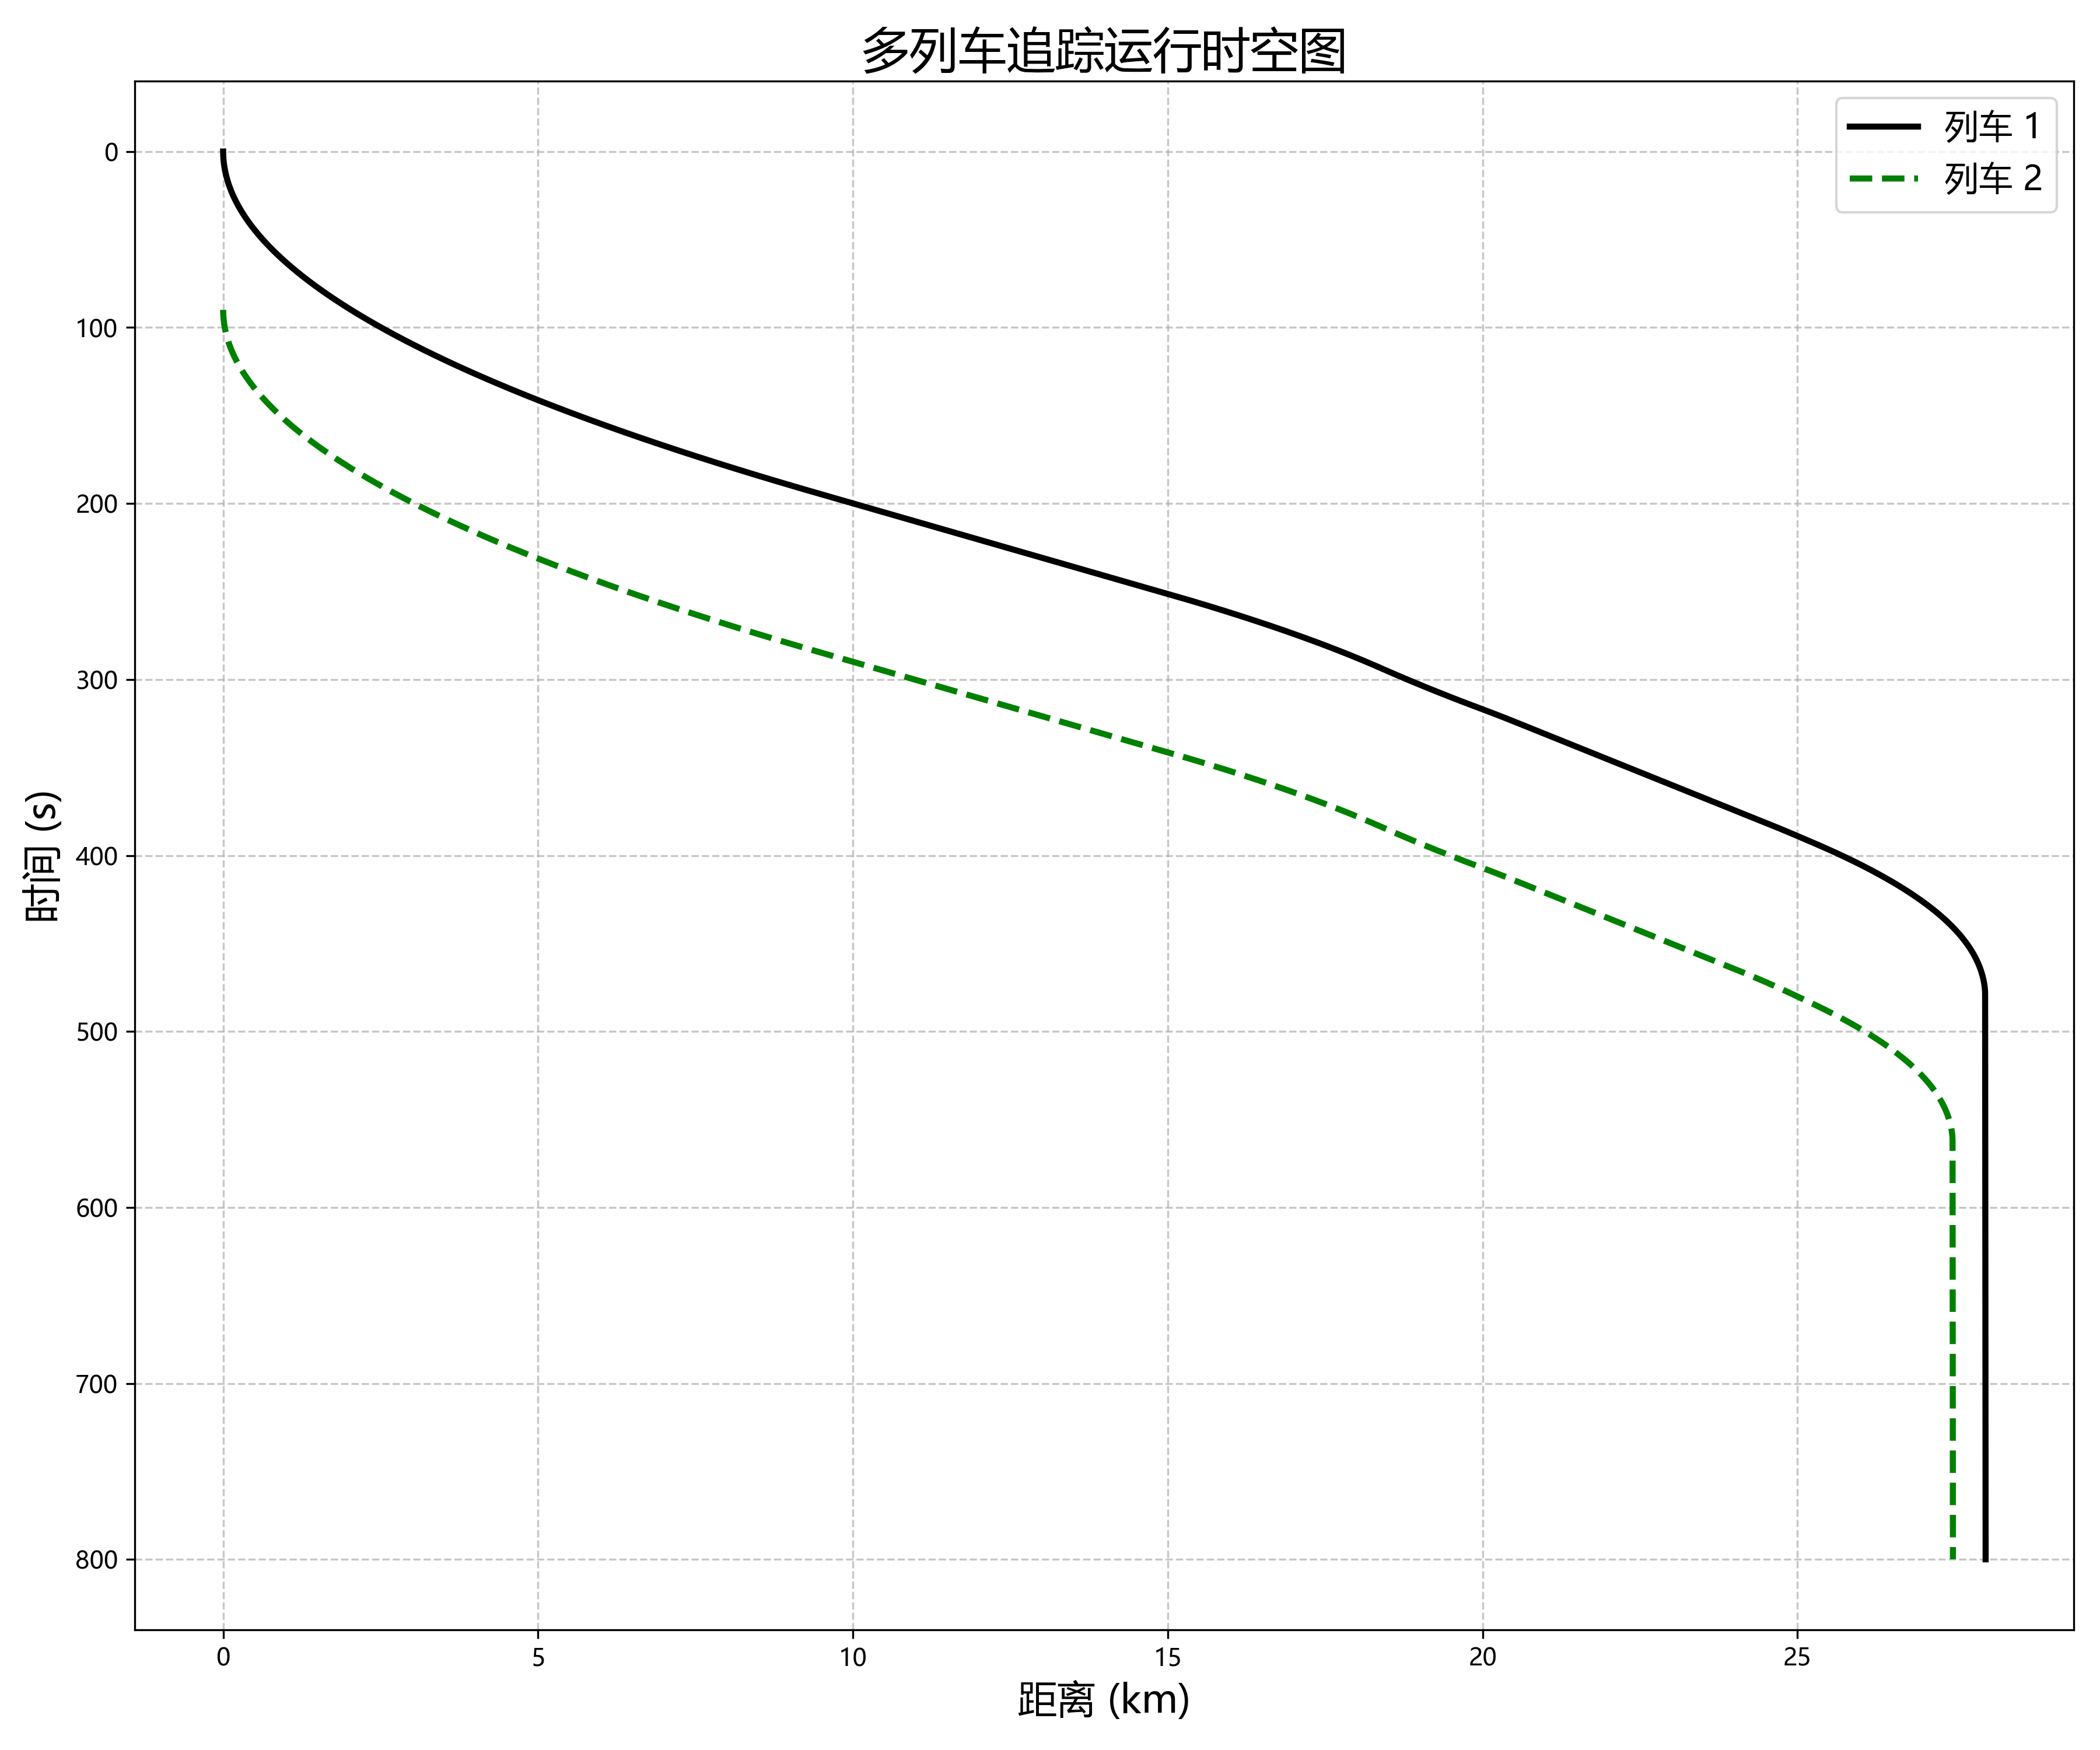
\includegraphics[width=0.48\textwidth]{headway_90s.png}
    \hfill
    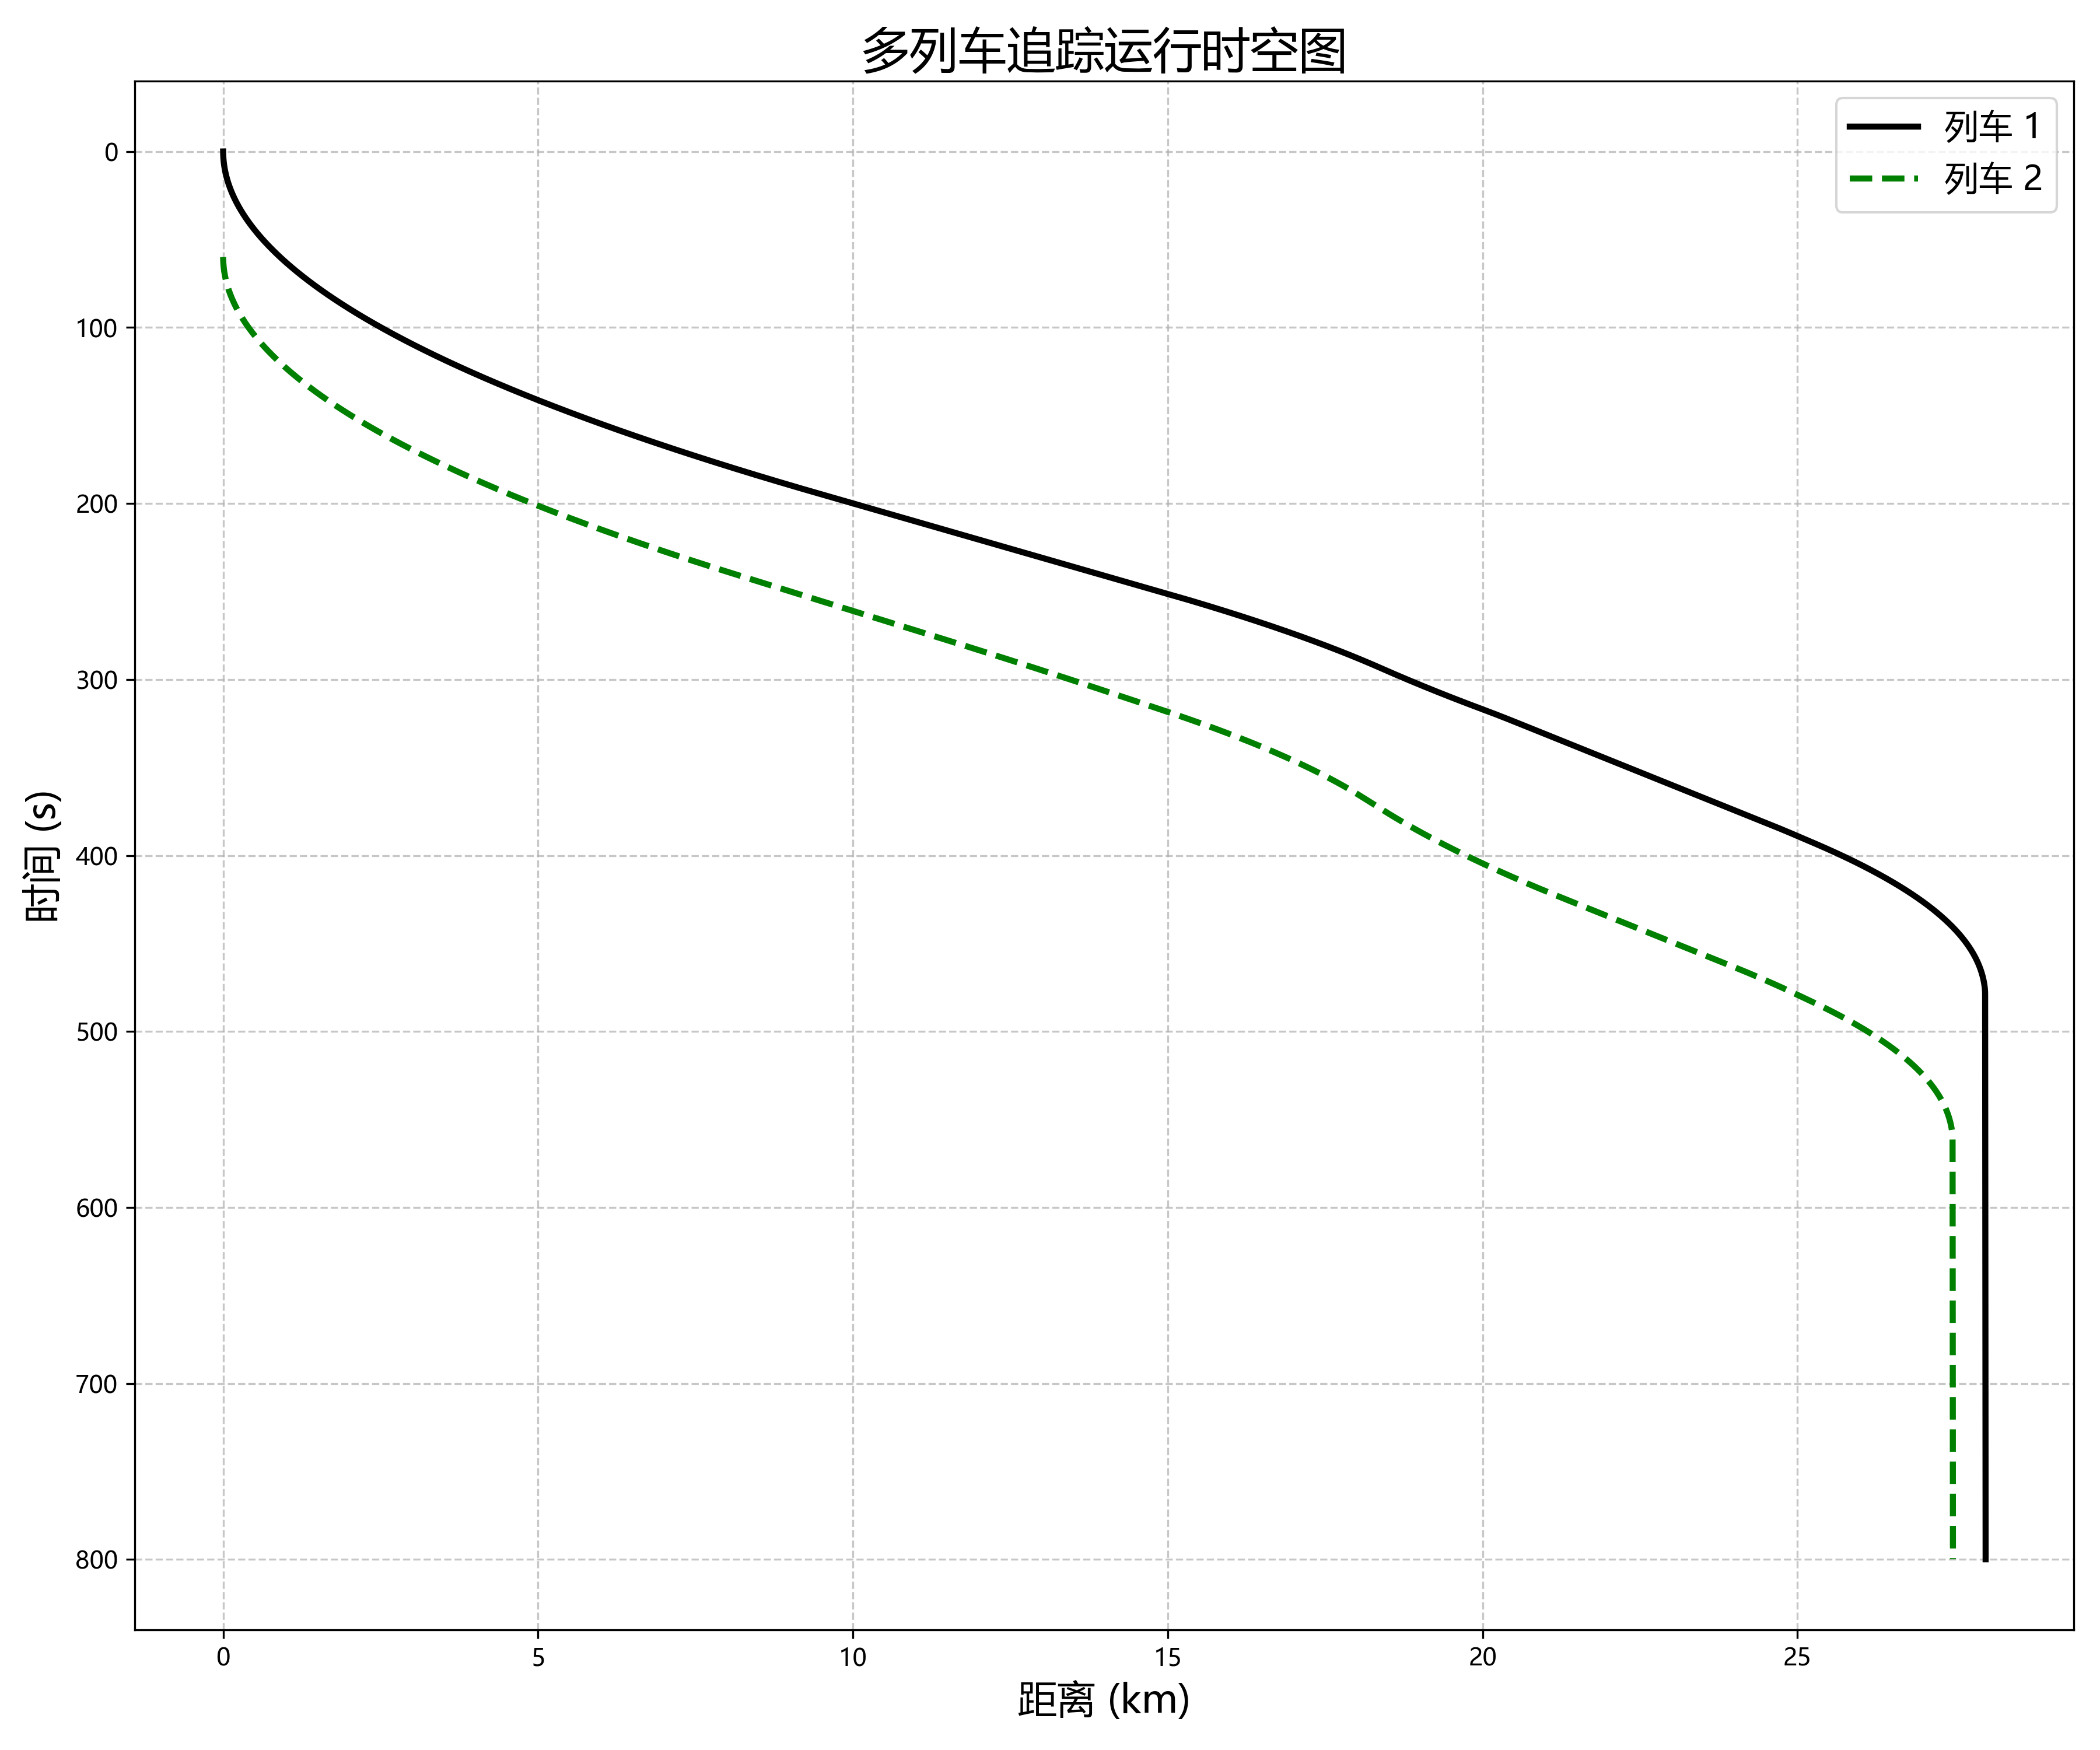
\includegraphics[width=0.48\textwidth]{headway_60s.png}
    \caption{过密间隔(90s, 左)与极端间隔(60s, 右)时空图对比}
    \label{fig:headway_compare2}
\end{figure}

如图\ref{fig:headway_compare1}和\ref{fig:headway_compare2}所示,随着发车间隔从180秒逐步缩短,后车(绿色虚线)的运行轨迹因受到前车压制而变得越来越陡峭,其平均运行速度显著下降。在180s时,两条曲线几乎平行,后车运行不受影响。在120s时,“速度压制”现象开始显现。当间隔缩短至90s和60s时,后车的速度被严重限制,线路的整体运输效率大幅降低。

作为补充,我们还进行了10秒极端发车间隔的仿真(见图\ref{fig:headway_extreme})。在这种情况下,后车几乎从发车开始就受到前车的严重压制,其速度曲线被完全“压平”,全程低速运行。这生动地说明,盲目压缩发车间隔并不能无限提升线路通过能力,当间隔小到一定程度后,反而会因严重的“速度压制”而导致整个线路的运行效率急剧下降。

\begin{figure}[h!]
    \centering
    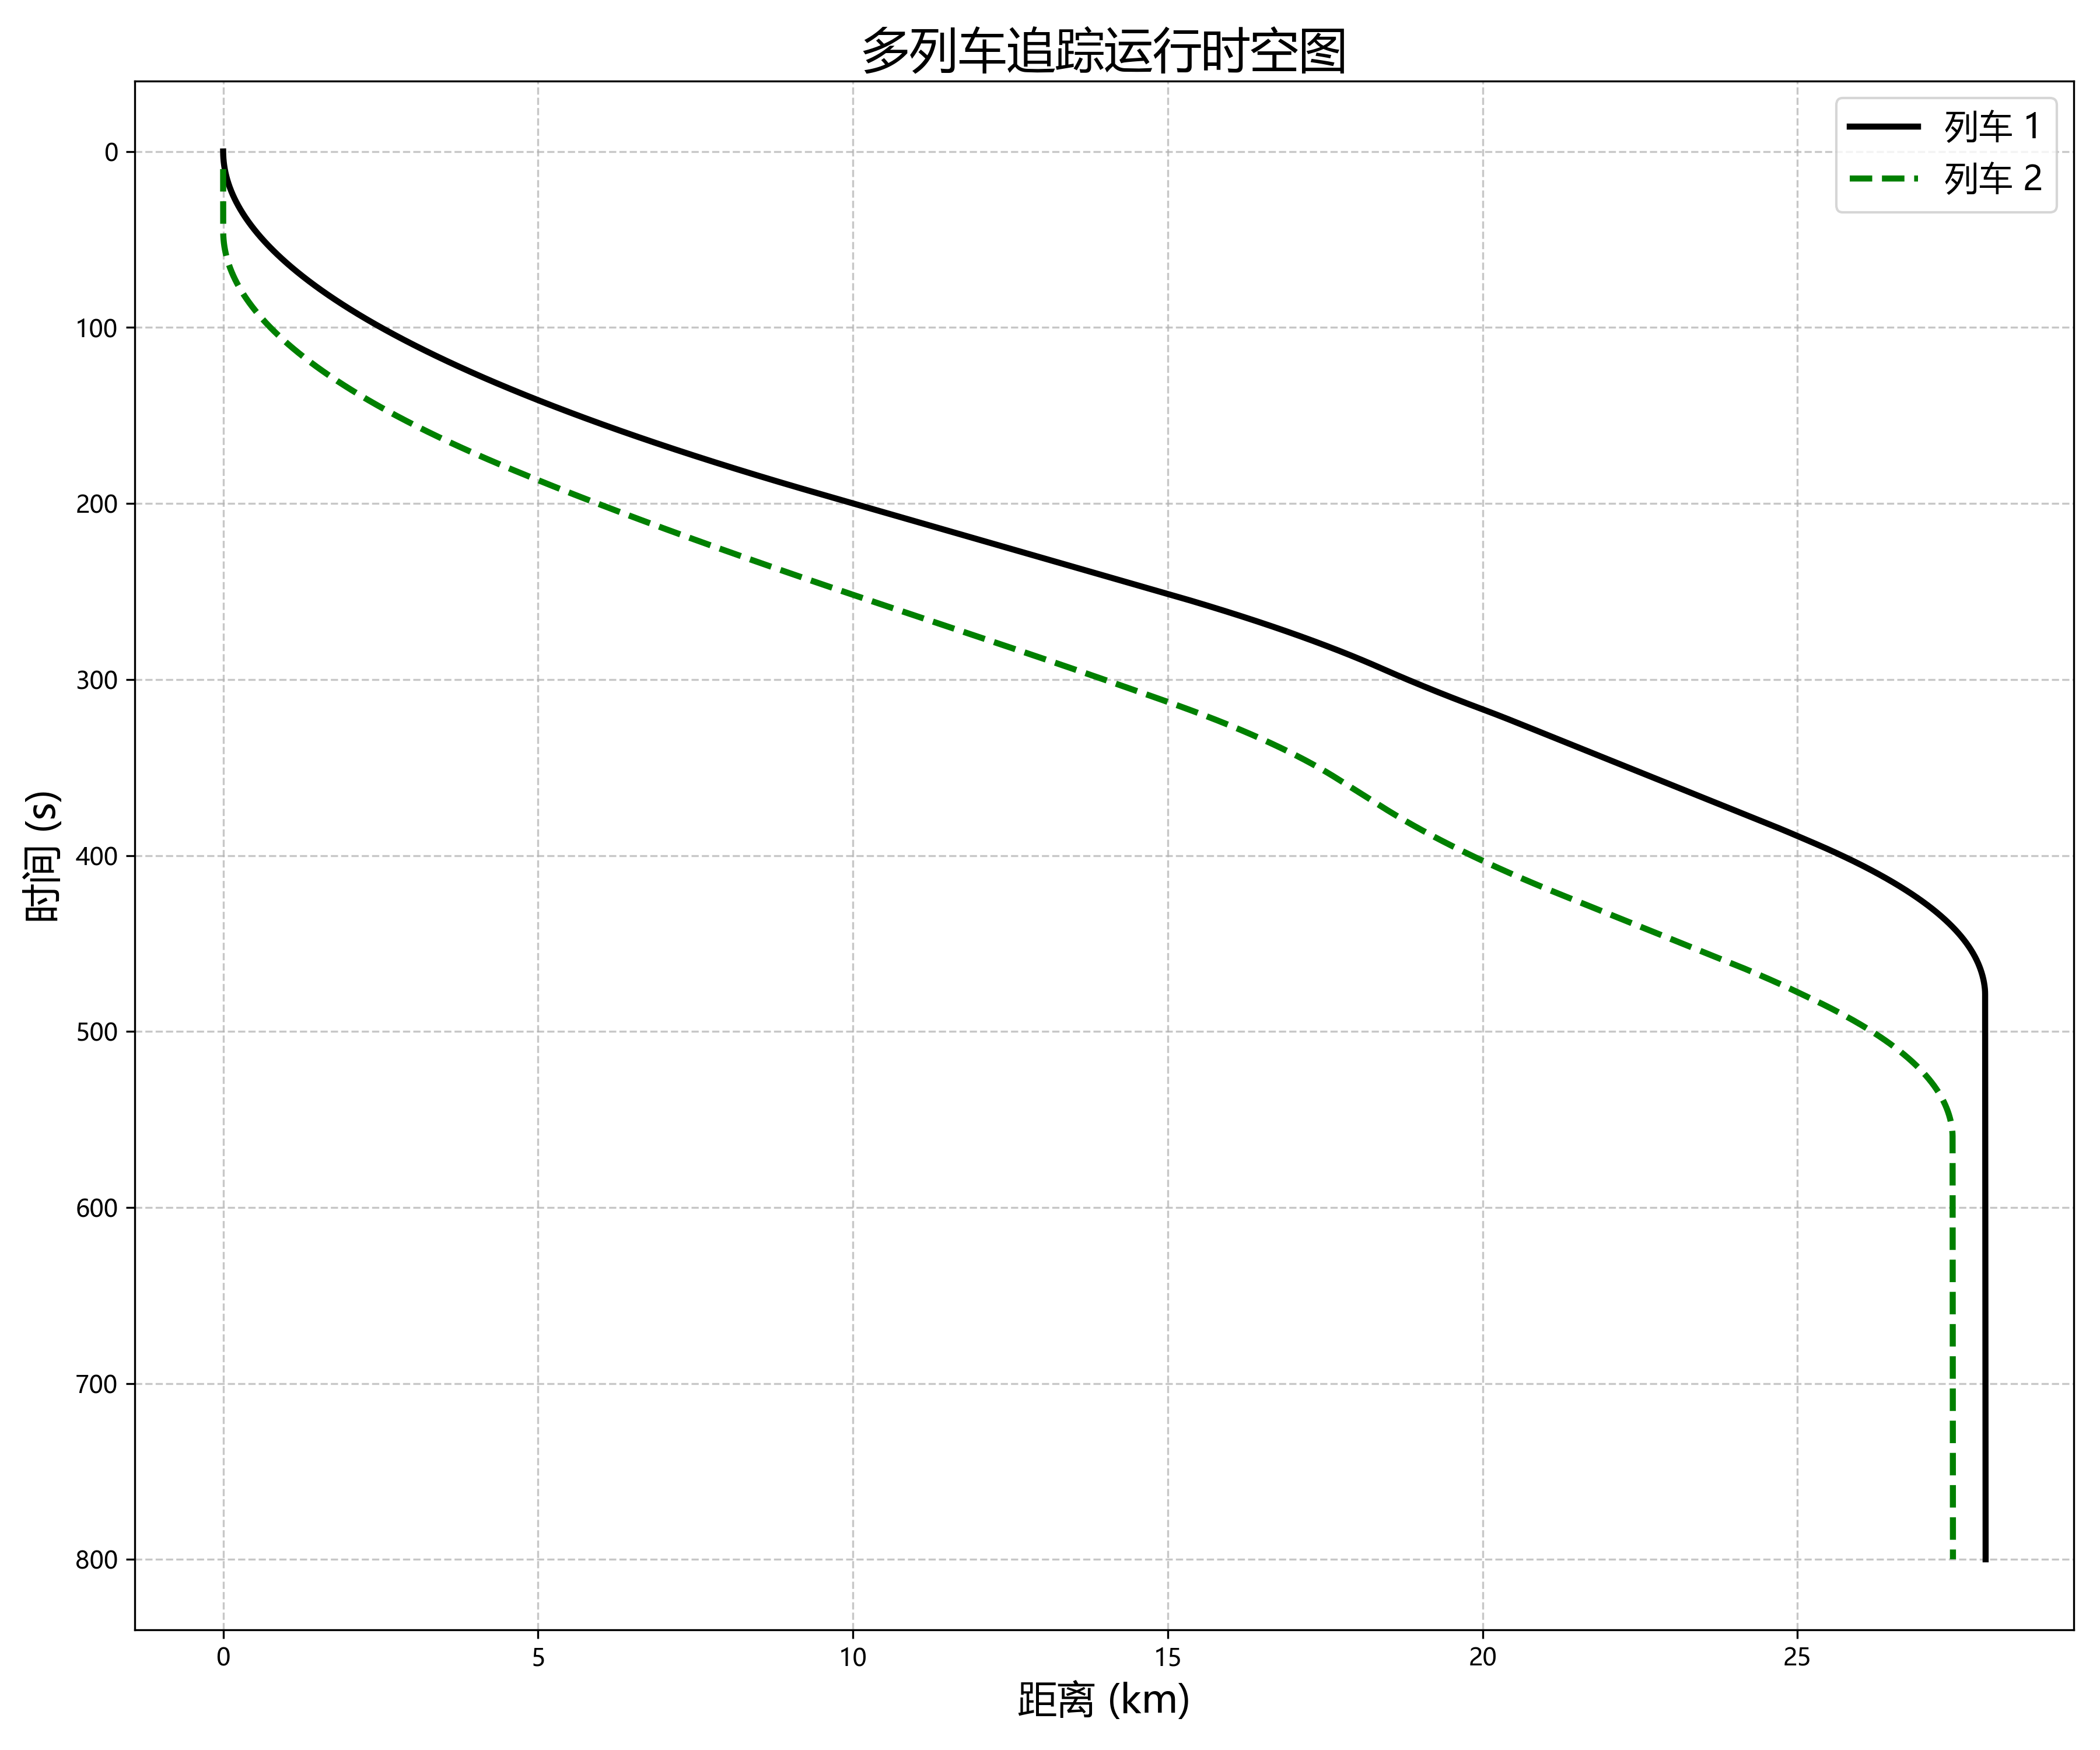
\includegraphics[width=0.8\textwidth]{headway_10s.png}
    \caption{极端发车间隔(10s)下的时空图}
    \label{fig:headway_extreme}
\end{figure}

实验结果表明,在当前仿真条件下,120秒是兼顾安全与效率的最小高效行车间隔。这一定量分析直观地展示了基于移动闭塞原理的列控系统在提升线路通过能力方面的巨大优势,同时也揭示了其物理和安全的极限。

% --- 结论 ---
\section{结论}
本课程实验成功地设计并实现了一个功能模块化的列车运行控制仿真平台。通过对单列车ATP/ATO、CTCS-3级动态授权和多列车追踪三个核心场景的仿真与分析,得出以下结论:
\begin{enumerate}
    \item 仿真平台准确复现了ATP系统基于MRSP和动态制动曲线簇构建“安全包络”的核心原理,验证了其在复杂场景下保障行车安全的能力。
    \item 对比实验量化了不同ATO驾驶策略的性能差异,证明了“节能优先”策略在牺牲有限运行时间的情况下,能够大幅降低能源消耗,为智能驾驶优化提供了数据支持。
    \item 通过模拟RBC与车载设备的交互,成功展示了CTCS-3级“移动授权”的工作机制,验证了其在提升高速线路运行效率和响应突发事件方面的优越性。
    \item 系列化的多列车追踪实验,直观地揭示了行车间隔与线路通行能力之间的非线性关系,并定量地探究出了特定条件下的最小高效行车间隔,为理解移动闭塞理论提供了实践依据。
\end{enumerate}
综上,本次实验将抽象的列控理论与动态的可视化结果相结合,深化了对现代列车运行控制系统安全性、高效性和智能性的理解。

% --- 参考文献 ---
\section{参考文献}
\begin{thebibliography}{9}
    \bibitem{lec_main} 李蔚. (2025). 《列车运行控制系统》. 中南大学交通运输工程学院课程资料.
\end{thebibliography}

% --- 附录 ---
\section*{附录}
\appendix
\section{仿真程序源代码}
本实验的全部Python源代码及相关文件已托管至GitHub仓库,可通过以下链接访问:
\href{https://github.com/Gan0819Han/Train_operation_control_system}{\texttt{https://github.com/Gan0819Han/Train\_operation\_control\_system}}

\end{document}
